% Gabarit pandoc des corrigés publiés (brut et guidé). Contenu sans marque ni nom de site.
% Compilation : lualatex (latexmk -lualatex).
% Le Markdown reste la source unique : ne pas éditer ce fichier .tex à la main.
\documentclass[11pt,a4paper]{article}

% --- Moteur, polices (Latin Modern) et langue ---------------------------------
\usepackage{iftex}
\ifLuaTeX\else\errmessage{Ce document se compile avec lualatex}\fi
\usepackage{amsmath,amssymb,mathtools}
\usepackage{fontspec}
% mathrm=sym : \mathrm prend ses glyphes dans la police mathématique (ℓ, μ, Ω), comme KaTeX.
\usepackage[math-style=TeX,bold-style=TeX,mathrm=sym]{unicode-math}
% Repli pour les glyphes absents de Latin Modern (indices et exposants Unicode,
% flèches, filets des schémas en texte, symboles) : DejaVu, puis Latin Modern Math
% (ℓ, lettres mathématiques Unicode des légendes).
\directlua{
  luaotfload.add_fallback("repliTexte", {"DejaVuSerif:mode=harf;", "DejaVuSans:mode=harf;", "file:latinmodern-math.otf:mode=harf;"})
  luaotfload.add_fallback("repliMono", {"DejaVuSansMono:mode=harf;", "DejaVuSans:mode=harf;", "file:latinmodern-math.otf:mode=harf;"})
}
\setmainfont{Latin Modern Roman}[RawFeature={fallback=repliTexte}]
\setsansfont{Latin Modern Sans}[RawFeature={fallback=repliTexte}]
\setmonofont{Latin Modern Mono}[RawFeature={fallback=repliMono}]
\setmathfont{Latin Modern Math}
\usepackage[french]{babel}
\frenchsetup{SmallCapsFigTabCaptions=false}

% --- Mise en page --------------------------------------------------------------
\usepackage[a4paper,margin=2.2cm,headheight=14pt,footskip=1.2cm]{geometry}
\usepackage{microtype}
\setlength{\emergencystretch}{4em}
\tolerance=1500
\setlength{\parindent}{0pt}
\setlength{\parskip}{0.55\baselineskip plus 2pt minus 1pt}
\usepackage{xcolor}
% Gris nommés : babel-french rend « ! » actif dans le document.
\definecolor{gris2}{gray}{0.98}
\definecolor{gris3}{gray}{0.97}
\definecolor{gris5}{gray}{0.95}
\definecolor{gris35}{gray}{0.65}
\definecolor{gris40}{gray}{0.60}
\definecolor{gris45}{gray}{0.55}
\definecolor{gris50}{gray}{0.50}
\definecolor{gris55}{gray}{0.45}
\definecolor{gris60}{gray}{0.40}
\definecolor{gris65}{gray}{0.35}
\definecolor{gris70}{gray}{0.30}
\definecolor{gris80}{gray}{0.20}
\definecolor{gris85}{gray}{0.15}
\usepackage{graphicx}
\usepackage{float}
\usepackage{caption}
\captionsetup{font=small,labelformat=empty,justification=centering}
\usepackage{booktabs,longtable,array,multirow,calc}
\usepackage{siunitx}
\sisetup{locale=FR}
\usepackage[version=4]{mhchem}
\usepackage{listings}
\usepackage{fancyhdr}
\usepackage{lastpage}
\usepackage[most]{tcolorbox}
\usepackage{enumitem}
\setlist{nosep,leftmargin=*,topsep=2pt}
\usepackage[hidelinks,unicode]{hyperref}
\usepackage{bookmark}
\hypersetup{pdftitle={X-ENS PC — Mathématiques 2026},pdfauthor={Rédigé par IA},pdfcreator={LaTeX},pdfsubject={Corrigé guidé}}
\usepackage{xurl}

% --- Pandoc : listes, tableaux, figures ----------------------------------------
\providecommand{\passthrough}[1]{#1}
\providecommand{\tightlist}{\setlength{\itemsep}{0pt}\setlength{\parskip}{0pt}}

\makeatletter
\def\maxwidth{\ifdim\Gin@nat@width>\linewidth\linewidth\else\Gin@nat@width\fi}
\def\maxheight{\ifdim\Gin@nat@height>0.55\textheight 0.55\textheight\else\Gin@nat@height\fi}
\makeatother
\setkeys{Gin}{width=\maxwidth,height=\maxheight,keepaspectratio}
\setcounter{secnumdepth}{-\maxdimen}
\providecommand{\pandocbounded}[1]{#1}

% --- Code (listings) -----------------------------------------------------------
\lstset{
  basicstyle=\ttfamily\small,
  columns=fullflexible,
  keepspaces=true,
  breaklines=true,
  breakatwhitespace=false,
  postbreak=\mbox{\textcolor{gris50}{$\hookrightarrow$}\space},
  frame=single,
  rulecolor=\color{gris35},
  framesep=4pt,
  xleftmargin=5pt,xrightmargin=5pt,
  backgroundcolor=\color{gris3},
  keywordstyle=\bfseries,
  commentstyle=\color{gris65},
  stringstyle=\color{gris80},
  showstringspaces=false,
  tabsize=4,
  extendedchars=true,
  aboveskip=6pt,belowskip=6pt,
}

% --- Macros des corrigés (KaTeX ↔ LaTeX) ---------------------------------------
% Les corrigés sont écrits pour KaTeX : on définit ici ce que KaTeX connaît et
% que LaTeX n'a pas, sans jamais retoucher le Markdown.
\providecommand{\R}{\mathbb{R}}
\providecommand{\N}{\mathbb{N}}
\providecommand{\Z}{\mathbb{Z}}
\providecommand{\Q}{\mathbb{Q}}
\providecommand{\C}{\mathbb{C}}
\providecommand{\dd}{\mathrm{d}}
\providecommand{\llbracket}{\lBrack}
\providecommand{\rrbracket}{\rBrack}
\providecommand{\lBrace}{\lbrace}
\providecommand{\rBrace}{\rbrace}
\providecommand{\Box}{\square}
\providecommand{\Diamond}{\lozenge}
\providecommand{\varnothing}{\emptyset}
\providecommand{\argmax}{\operatorname*{arg\,max}}
\providecommand{\argmin}{\operatorname*{arg\,min}}
\renewcommand{\leq}{\leqslant}
\renewcommand{\geq}{\geqslant}

% Équation hors texte : réduite à la largeur de la ligne si elle déborde.
\newsavebox{\boiteequation}
\newcommand{\equationajustee}[1]{%
  \sbox{\boiteequation}{$\displaystyle #1$}%
  \ifdim\wd\boiteequation>\linewidth
    \[\resizebox{\linewidth}{!}{\usebox{\boiteequation}}\]%
  \else
    \[#1\]%
  \fi}

% --- Encadrés pédagogiques (sobres, lisibles en noir et blanc) -----------------
\tcbset{
  encadre/.style={
    enhanced,breakable,sharp corners,
    colback=white,colframe=gris55,
    boxrule=0.4pt,leftrule=2.2pt,
    left=6pt,right=6pt,top=3pt,bottom=3pt,
    before skip=6pt,after skip=6pt,
    fonttitle=\bfseries\small,coltitle=black,
    attach title to upper,after title={\quad},
    parbox=false,
  }
}
\newtcolorbox{indication}[1]{encadre,colframe=gris45,colback=gris2,title={Indication~#1}}
\newtcolorbox{methode}{encadre,colframe=gris70,title={Méthode}}
\newtcolorbox{piege}{encadre,colframe=gris85,boxrule=0.8pt,leftrule=2.2pt,title={Piège}}
\newtcolorbox{jury}{encadre,colframe=gris60,colback=gris5,title={Jury}}
\newtcolorbox{encadrenote}{encadre,colframe=gris40}

% --- Titres de section ---------------------------------------------------------
\usepackage{titlesec}
\titleformat{\section}{\Large\bfseries}{}{0pt}{}
\titleformat{\subsection}{\large\bfseries}{}{0pt}{}
\titleformat{\subsubsection}{\normalsize\bfseries}{}{0pt}{}
\titlespacing*{\section}{0pt}{14pt plus 4pt minus 2pt}{6pt}
\titlespacing*{\subsection}{0pt}{10pt plus 3pt minus 2pt}{4pt}
\titlespacing*{\subsubsection}{0pt}{8pt plus 2pt minus 2pt}{2pt}

% --- En-tête et pied de page ---------------------------------------------------
\pagestyle{fancy}
\fancyhf{}
\fancyhead[L]{\small\textsc{Corrigé guidé} · X-ENS PC}
\fancyhead[R]{\small Maths PC 2026}
\fancyfoot[L]{\footnotesize Corrigé rédigé par IA, non officiel}
\fancyfoot[R]{\footnotesize \thepage\,/\,\pageref*{LastPage}}
\renewcommand{\headrulewidth}{0.4pt}
\renewcommand{\footrulewidth}{0pt}
\fancypagestyle{plain}{\fancyhf{}\fancyfoot[R]{\footnotesize \thepage\,/\,\pageref*{LastPage}}\fancyfoot[L]{\footnotesize Corrigé rédigé par IA, non officiel}\renewcommand{\headrulewidth}{0pt}}

\begin{document}
\thispagestyle{plain}
\begin{center}
  {\small\scshape Corrigé guidé}\par\smallskip
  {\LARGE\bfseries X-ENS PC — Mathématiques 2026\par}\medskip
  {\large X-ENS · PC · Maths PC · 2026\par}
\end{center}
\vspace{2pt}\hrule\vspace{8pt}

\emph{Corrigé rédigé par IA, non officiel. Signalez toute erreur.}

\hypertarget{pruxe9sentation-du-sujet}{%
\section{Présentation du sujet}\label{pruxe9sentation-du-sujet}}

\textbf{Thème.} Le sujet étudie deux modèles jouets du ferromagnétisme : des « spins » \(\sigma_i=\pm1\) indépendants et uniformes, pondérés par l'exponentielle d'une énergie. On veut calculer l'\textbf{énergie libre} (limite de \(\frac1N\ln\) d'une espérance) et l'\textbf{aimantation} (dérivée de l'énergie libre par rapport au champ \(h\)).

On met ensuite en évidence une \textbf{transition de phase} : pour \(\beta>\frac12\), l'énergie libre du modèle de champ moyen n'est plus dérivable en \(h=0\).

\textbf{Découpage.}

\begin{itemize}
\tightlist
\item
  \textbf{Partie I (Q1--Q8)} : un petit cours d'analyse convexe. Inégalité des pentes (Q1), stabilité de la convexité par limite simple (Q2--Q3), \textbf{convergence des dérivées} de fonctions convexes (Q4, l'outil clé du sujet), caractérisation par la hessienne (Q5--Q6), convexité de \(\phi(\lambda)=\ln E[e^{\lambda\cdot X}]\) (Q7--Q8).
\item
  \textbf{Partie II (Q9--Q18)} : modèle d'Ising sur un anneau de \(N\) spins. La fonction de partition devient la trace \(2^{-N}\operatorname{tr}(A^N)\) (méthode de la matrice de transfert). L'énergie libre limite est \(\ln\lambda(\beta,h)-\ln2\), où \(\lambda\) est la plus grande valeur propre, et l'aimantation limite s'obtient par Q4. Q17--Q18 regardent la limite basse température \(\beta\to+\infty\).
\item
  \textbf{Partie III (Q19--Q32)} : modèle de Curie--Weiss (champ moyen). Grandes déviations par Stirling (Q20--Q21), étude de \(\psi_{\beta,h}(x)=\beta x^2+hx-I(x)\) (Q23--Q25), dérivabilité de l'énergie libre \(g\) (Q27--Q29), aimantation (Q30--Q31), exposant critique \(\frac13\) (Q32).
\end{itemize}

\textbf{Notions mobilisées.} Convexité (définie par l'énoncé), dérivées partielles, hessienne, théorème de Schwarz, théorème des accroissements finis, réduction des matrices \(2\times2\), trace. Probabilités sur un univers fini (indépendance, formule de transfert, loi binomiale), formule de Stirling (rappelée), développements limités et séries entières usuelles, convergence simple et uniforme des suites de fonctions.

\textbf{Difficulté et longueur.} 32 questions en 4 heures, sans calculatrice. Les calculs sont courts ; la difficulté est dans la \textbf{rigueur des passages à la limite} (Q4, Q16, Q26, Q28, Q30) et dans les \textbf{preuves d'unicité} (Q24, Q25). On peut admettre les résultats des questions précédentes : chaque partie s'aborde indépendamment.

\textbf{Ce qu'en dit le rapport 2026.} Le jury relève que la rédaction « a parfois manqué de précision sur des notions fondamentales », en particulier la convexité et la justification de l'existence des limites ou des interversions de limites et de dérivées. La partie I « a posé d'assez grandes difficultés cette année et n'a parfois été que très peu traitée ». Il prévient enfin : « La stratégie de survoler le sujet en ne répondant qu'aux questions les plus simples ne peut aboutir à une note correcte. »

\textbf{Erratum à connaître.} Avec la fonction \(I\) de l'énoncé, la question 21 est fausse d'une constante : la vraie limite est \(I(x)+\ln2\). Le rapport 2026 le confirme : il manquait un terme en \(\ln 2\), sans conséquence pour la suite. La convergence admise après Q22 doit de même se lire \(G_N\to g-\ln2\). Cela ne change rien aux questions 23 à 32, qui portent sur des dérivées, des points de maximum ou des différences de valeurs de \(g\).

Devant une telle situation, la bonne conduite est de démontrer ce qui est vrai, de le dire en une phrase et de continuer. Autre coquille signalée par le jury : en Q5, il faut lire \(x\in\mathbb R^d\).

\textbf{Questions à ne pas laisser passer.} D'après le rapport, Q9, Q11 et Q12 ont été traitées dans presque toutes les copies : elles ne départagent pas, mais il faut les rédiger sans faute. Q1, Q2, Q3, Q7, Q19, Q20 et Q23 sont rapides. Q4 est un passage obligé : elle resservira en Q16, Q18 et Q30.

\textbf{Questions discriminantes.} Le jury signale des questions accessibles mais très peu traitées : Q22 (« assez peu difficile mais très peu traitée »), Q27 (« pas extrêmement difficile ») et Q31 (« très peu de résultats intermédiaires »). Elles rapportent beaucoup à qui ose la partie III. Q13 a été « très rarement traitée jusqu'au bout », et Q21, Q25, Q26, Q29 et Q32 ont été très peu traitées.

\textbf{Gestion du temps.} Environ 1 h pour la partie I, 1 h 15 pour la partie II, 1 h 45 pour la partie III, qui est la plus longue. Beaucoup de questions de la partie III, y compris la dernière, se font sans les parties précédentes : ne pas s'enliser dans la partie I.

\begin{center}\rule{0.5\linewidth}{0.5pt}\end{center}

\hypertarget{partie-i-convexituxe9}{%
\section{Partie I --- Convexité}\label{partie-i-convexituxe9}}

On établit les propriétés des fonctions convexes qui serviront à \textbf{échanger limite et dérivation}, puis on montre que \(\phi\) est convexe parce que sa hessienne est une matrice de covariance.

\hypertarget{question-1}{%
\subsection{Question 1}\label{question-1}}

\begin{indication}{1}

Commencer par comparer les pentes des cordes issues de \(x\) : écrire \(x+s\) comme barycentre de \(x\) et de \(x+t\), pour \(0<s\leqslant t\).

\end{indication}

\begin{indication}{2}

Le taux d'accroissement à droite \(s\mapsto\frac{g(x+s)-g(x)}{s}\) est monotone : dans quel sens ? Sa limite en \(0^+\) est alors une borne pour toutes ses valeurs.

\end{indication}

\hypertarget{solution}{%
\subsubsection{Solution}\label{solution}}

Soit \(h>0\). Pour \(0<s\leqslant t\), posons \(\alpha=s/t\in\,]0,1]\). On a \(x+s=\alpha(x+t)+(1-\alpha)x\), donc, par la définition de la convexité,
\equationajustee{g(x+s)\leqslant\alpha\,g(x+t)+(1-\alpha)\,g(x).}
En retranchant \(g(x)\) et en divisant par \(s>0\) :
\equationajustee{\frac{g(x+s)-g(x)}{s}\leqslant\frac{g(x+t)-g(x)}{t}.}
Le taux \(\tau_+(s)=\frac{g(x+s)-g(x)}{s}\) est donc croissant sur \(]0,+\infty[\).

De même, \(x-s=\alpha(x-t)+(1-\alpha)x\) donne
\equationajustee{g(x-s)-g(x)\leqslant\frac st\big(g(x-t)-g(x)\big).}
Après division par \(s\) et changement de signe, le taux \(\tau_-(s)=\frac{g(x)-g(x-s)}{s}\) est \textbf{décroissant} en \(s\).

Comme \(g\) est dérivable en \(x\) (et seulement supposée telle en ce point), \(\tau_+(s)\) et \(\tau_-(s)\) tendent vers \(g'(x)\) quand \(s\to0^+\).

Pour \(0<s\leqslant h\), la monotonie donne
\equationajustee{\tau_-(h)\leqslant\tau_-(s)\qquad\text{et}\qquad\tau_+(s)\leqslant\tau_+(h).}
Dans chacune de ces inégalités, le membre de gauche et le membre de droite ont une limite quand \(s\to0^+\) (l'un est constant). Le passage à la limite dans les inégalités larges donne \(\tau_-(h)\leqslant g'(x)\) et \(g'(x)\leqslant\tau_+(h)\) :
\equationajustee{\boxed{\frac{g(x)-g(x-h)}{h}\leqslant g'(x)\leqslant\frac{g(x+h)-g(x)}{h}}}

\begin{figure}[H]
\centering
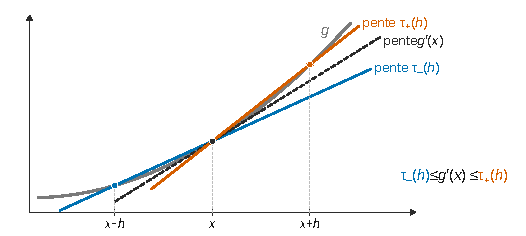
\includegraphics{figures/q01-pentes-cordes.pdf}
\caption*{Figure 1 --- Inégalité des pentes : pour g convexe, la corde de gauche
(pente τ₋(h)) est moins inclinée que la tangente en x, elle-même moins
inclinée que la corde de droite (pente τ₊(h))}
\end{figure}

\begin{methode}

Pour une fonction convexe, « la pente des cordes croît ». C'est la forme la plus utile de la convexité : elle donne aussitôt l'encadrement de la dérivée par les pentes à gauche et à droite.

\end{methode}

\begin{piege}

Le rapport 2026 signale des passages à la limite incomplets : on fait tendre \(s\) vers \(0^+\) dans \textbf{tous} les membres de l'inégalité, après avoir vérifié que chacun a une limite. Ici l'un est constant, l'autre tend vers \(g'(x)\) par la seule dérivabilité en \(x\).

\end{piege}

\begin{jury}

Le rapport 2026 rappelle que « la fonction en question n'était supposée dérivable qu'en un seul point (et pas plus) » et qu'on attendait « la démonstration complète du lemme des pentes » à partir de la définition de l'énoncé. Les copies qui ont invoqué un résultat de cours fondé sur ce lemme n'ont obtenu qu'une partie des points.

\end{jury}

\hypertarget{question-2}{%
\subsection{Question 2}\label{question-2}}

\begin{indication}{1}

La convexité est une famille d'inégalités larges entre valeurs de la fonction en trois points. Que deviennent ces inégalités par passage à la limite simple ?

\end{indication}

\hypertarget{solution-1}{%
\subsubsection{Solution}\label{solution-1}}

Soient \(x,y\in\mathbb R\) et \(\alpha\in[0,1]\). Pour tout \(n\),
\equationajustee{f_n(\alpha x+(1-\alpha)y)\leqslant\alpha f_n(x)+(1-\alpha)f_n(y).}
Les trois suites \((f_n(\alpha x+(1-\alpha)y))_n\), \((f_n(x))_n\) et \((f_n(y))_n\) convergent, par convergence simple. Le passage à la limite dans l'inégalité large donne
\equationajustee{f(\alpha x+(1-\alpha)y)\leqslant\alpha f(x)+(1-\alpha)f(y).}
\textbf{\(f\) est convexe.}

\hypertarget{question-3}{%
\subsection{Question 3}\label{question-3}}

\begin{indication}{1}

Chercher une suite de fonctions convexes régulières qui « arrondit » une fonction convexe présentant un point anguleux.

\end{indication}

\begin{indication}{2}

La valeur absolue est la candidate naturelle ; on peut l'approcher par une racine carrée \(\sqrt{x^2+\varepsilon_n}\).

\end{indication}

\hypertarget{solution-2}{%
\subsubsection{Solution}\label{solution-2}}

Pour \(n\in\mathbb N\), posons \(f_n(x)=\sqrt{x^2+\frac1{n+1}}\). Le radicande est minoré par \(\frac1{n+1}>0\).

La racine carrée est de classe \(\mathcal C^\infty\) sur \(]0,+\infty[\), donc \(f_n\) est de classe \(\mathcal C^2\) sur \(\mathbb R\), avec
\equationajustee{f_n'(x)=\frac{x}{\sqrt{x^2+\frac1{n+1}}}}
et
\equationajustee{f_n''(x)=\frac{\frac1{n+1}}{\big(x^2+\frac1{n+1}\big)^{3/2}}>0 .}

\emph{Convexité.} La hessienne de \(f_n\) (matrice \(1\times1\) égale à \(f_n''(x)\)) est symétrique positive en tout point. Par Q6 avec \(d=1\), \textbf{\(f_n\) est convexe} ; elle est dérivable.

\emph{Convergence.} Pour \(x\) fixé, \(x^2+\frac1{n+1}\to x^2\) et la racine carrée est continue sur \([0,+\infty[\), donc \(f_n(x)\to\sqrt{x^2}=|x|\).

\textbf{La limite simple \(f=|\cdot|\) n'est pas dérivable en \(0\)} : son taux d'accroissement en \(0\) vaut \(1\) à droite et \(-1\) à gauche.

\begin{jury}

Le rapport 2026 : « Dans un certain nombre de copies, les justifications de la convexité ou de la convergence étaient absentes. » Il faut vérifier, pour chaque \(f_n\), qu'elle est convexe \textbf{et} dérivable, puis établir la convergence simple.

\end{jury}

\begin{methode}

Le jury note que certaines copies ont pris un contre-exemple dans la suite du sujet, « qui n'était pas le plus simple ». Il cite la question 19 ; la suite qui convient est plutôt celle des \(g_\beta\) de Q17, convexes, dérivables et tendant simplement vers \(|\cdot|\).

\end{methode}

\hypertarget{question-4}{%
\subsection{Question 4}\label{question-4}}

\begin{indication}{1}

Encadrer \(f_n'(x)\) par Q1 avec un pas \(h\), puis faire tendre \(n\) vers l'infini à \(h\) fixé.

\end{indication}

\begin{indication}{2}

L'ordre des choix compte : on choisit d'abord \(h\) grâce à la dérivabilité de \(f\) en \(x\), puis un rang \(n_0\) grâce à la convergence simple en trois points.

\end{indication}

\hypertarget{solution-3}{%
\subsubsection{Solution}\label{solution-3}}

Soit \(\varepsilon>0\). Comme \(f\) est dérivable en \(x\), on fixe \(h>0\) tel que
\equationajustee{\frac{f(x)-f(x-h)}{h}\geqslant f'(x)-\varepsilon}
et
\equationajustee{\frac{f(x+h)-f(x)}{h}\leqslant f'(x)+\varepsilon.}
Le pas \(h\) étant fixé, la convergence simple en \(x-h\), \(x\) et \(x+h\) fournit \(n_0\) tel que, pour \(n\geqslant n_0\),
\equationajustee{\frac{f_n(x)-f_n(x-h)}{h}\geqslant\frac{f(x)-f(x-h)}{h}-\varepsilon}
et
\equationajustee{\frac{f_n(x+h)-f_n(x)}{h}\leqslant\frac{f(x+h)-f(x)}{h}+\varepsilon.}
La question 1, appliquée à \(f_n\) (convexe et dérivable en \(x\)), encadre \(f_n'(x)\) entre ces deux taux. On enchaîne les minorations d'une part, les majorations d'autre part : pour \(n\geqslant n_0\),
\equationajustee{\begin{aligned}
f_n'(x)&\geqslant\frac{f_n(x)-f_n(x-h)}{h}\geqslant f'(x)-2\varepsilon,\\
f_n'(x)&\leqslant\frac{f_n(x+h)-f_n(x)}{h}\leqslant f'(x)+2\varepsilon.
\end{aligned}}
Ainsi \(|f_n'(x)-f'(x)|\leqslant2\varepsilon\) pour \(n\geqslant n_0\). Ceci établit à la fois l'existence de la limite et sa valeur :
\equationajustee{\boxed{\lim_{n\to\infty}f_n'(x)=f'(x)}}

\begin{jury}

Le rapport 2026 souligne qu'on n'était pas, a priori, dans une situation permettant d'utiliser la convergence dominée pour intervertir les limites : « Il fallait donc, par exemple, justifier l'existence de la limite des \(f'_n(x)\). » La rédaction en \(\varepsilon\) ci-dessus établit existence et valeur d'un même mouvement.

\end{jury}

\begin{piege}

Soustraire des encadrements. De \(a\leqslant u\leqslant b\) et \(a'\leqslant v\leqslant b'\), on tire \(a-b'\leqslant u-v\leqslant b-a'\), et non \(a-a'\leqslant u-v\leqslant b-b'\). Le jury relève ce manque de rigueur ; on l'évite en enchaînant séparément les minorations et les majorations, comme ci-dessus.

\end{piege}

\begin{methode}

Ce résultat est le moteur du sujet : \textbf{la convexité permet de dériver une limite simple}. Il resservira en Q16, Q18 et Q30. Retenir les hypothèses : \(f_n\) convexes et dérivables, convergence simple, \(f\) dérivable au point considéré.

\end{methode}

\hypertarget{question-5}{%
\subsection{Question 5}\label{question-5}}

\begin{indication}{1}

Suivre l'indication : la fonction \(t\mapsto g(x+tu)\) est convexe sur \(\mathbb R\). Que dit Q1 de sa dérivée ?

\end{indication}

\begin{indication}{2}

Calculer la dérivée seconde de \(t\mapsto g(x+tu)\) par la règle de la chaîne et l'évaluer en \(t=0\).

\end{indication}

\hypertarget{solution-4}{%
\subsubsection{Solution}\label{solution-4}}

(On lit \(x\in\mathbb R^d\).) Rappelons qu'une matrice \(S\in\mathcal M_d(\mathbb R)\) est symétrique positive si \({}^tS=S\) et \({}^tu\,S\,u\geqslant0\) pour tout \(u\in\mathbb R^d\).

\emph{Symétrie.} \(g\) étant de classe \(\mathcal C^2\), sa hessienne \(\nabla^2g(x)\) est symétrique (théorème de Schwarz).

\emph{Positivité.} Soit \(u\in\mathbb R^d\) et \(\gamma(t)=g(x+tu)\), de classe \(\mathcal C^2\) sur \(\mathbb R\). Par la règle de la chaîne,
\equationajustee{\gamma'(t)=\sum_{i=1}^du_i\,\partial_ig(x+tu)}
et
\equationajustee{\begin{aligned}
\gamma''(t)&=\sum_{i,j}u_iu_j\,\partial_{ij}g(x+tu)\\
&={}^tu\,\nabla^2g(x+tu)\,u.
\end{aligned}}
\(\gamma\) est convexe, car \(x+(\alpha s+(1-\alpha)t)u=\alpha(x+su)+(1-\alpha)(x+tu)\).

Pour \(s<t\), la question 1 appliquée à \(\gamma\) en \(s\) et en \(t\), avec le pas \(t-s\), donne
\equationajustee{\gamma'(s)\leqslant\frac{\gamma(t)-\gamma(s)}{t-s}\leqslant\gamma'(t).}
\(\gamma'\) est donc croissante, d'où \(\gamma''\geqslant0\). En \(t=0\), \({}^tu\,\nabla^2g(x)\,u\geqslant0\) pour tout \(u\).

\textbf{La hessienne de \(g\) en \(x\) est symétrique positive.}

\begin{piege}

Le rapport 2026 note qu'« un nombre important de copies ont utilisé des caractérisations erronées » de la notion de matrice symétrique positive. Des coefficients positifs, ou une diagonale positive, ne suffisent pas : la définition est \({}^tS=S\) et \({}^tu\,S\,u\geqslant0\) pour tout \(u\) (ou, de façon équivalente, spectre réel positif).

\end{piege}

\begin{methode}

Restreindre une fonction de plusieurs variables à une droite \(t\mapsto x+tu\) ramène les questions de convexité et de positivité de la hessienne à la dimension 1.

\end{methode}

\hypertarget{question-6}{%
\subsection{Question 6}\label{question-6}}

\begin{indication}{1}

Même restriction qu'en Q5, au segment \([x,y]\) : il faut montrer qu'une fonction d'une variable de dérivée croissante est convexe.

\end{indication}

\begin{indication}{2}

Comparer, par le théorème des accroissements finis, les pentes des cordes sur \([0,\alpha]\) et sur \([\alpha,1]\).

\end{indication}

\hypertarget{solution-5}{%
\subsubsection{Solution}\label{solution-5}}

Soient \(x,y\in\mathbb R^d\) et \(\gamma(t)=g(x+t(y-x))\) pour \(t\in[0,1]\). Il suffit d'établir \(\gamma(\alpha)\leqslant\alpha\gamma(1)+(1-\alpha)\gamma(0)\) pour tout \(\alpha\in[0,1]\). Comme en Q5,
\equationajustee{\gamma''(t)={}^t(y-x)\,\nabla^2g\big(x+t(y-x)\big)\,(y-x)\geqslant0,}
donc \(\gamma'\) est croissante sur \([0,1]\).

Soit donc \(\alpha\in[0,1]\). Si \(\alpha\in\{0,1\}\), l'inégalité cherchée est une égalité. Sinon, le théorème des accroissements finis sur \([0,\alpha]\) et sur \([\alpha,1]\) fournit \(c_1\in\,]0,\alpha[\) et \(c_2\in\,]\alpha,1[\) tels que
\equationajustee{\begin{aligned}
\frac{\gamma(\alpha)-\gamma(0)}{\alpha}&=\gamma'(c_1)\\
&\leqslant\gamma'(c_2)\\
&=\frac{\gamma(1)-\gamma(\alpha)}{1-\alpha}.
\end{aligned}}
En multipliant par \(\alpha(1-\alpha)>0\) :
\equationajustee{\begin{aligned}
(1-\alpha)\big(\gamma(\alpha)-\gamma(0)\big)&\leqslant\alpha\big(\gamma(1)-\gamma(\alpha)\big),\\
\gamma(\alpha)&\leqslant\alpha\,\gamma(1)+(1-\alpha)\,\gamma(0).
\end{aligned}}
Ainsi \(g(\alpha y+(1-\alpha)x)\leqslant\alpha g(y)+(1-\alpha)g(x)\) : \textbf{\(g\) est convexe.}

\begin{jury}

Question peu traitée selon le rapport 2026. La voie attendue est celle-ci : ramener la convexité de \(g\) à celle des fonctions \(t\mapsto g(x+tu)\), puis reprendre les arguments de la question précédente.

\end{jury}

\begin{piege}

Le théorème des accroissements finis s'applique sur un intervalle non trivial : les cas \(\alpha=0\) et \(\alpha=1\) se traitent à part. Ils sont immédiats, mais il faut les mentionner.

\end{piege}

\hypertarget{question-7}{%
\subsection{Question 7}\label{question-7}}

\begin{indication}{1}

\(X\) ne prend qu'un nombre fini de valeurs : écrire \(E[e^{\lambda\cdot X}]\) comme une somme finie par la formule de transfert.

\end{indication}

\begin{indication}{2}

Dériver une somme finie d'exponentielles ne demande aucun théorème ; il reste à dériver \(\ln\circ Z\) puis un quotient.

\end{indication}

\hypertarget{solution-6}{%
\subsubsection{Solution}\label{solution-6}}

Soit \(V\subset\mathbb R^d\) l'ensemble \textbf{fini} des valeurs de \(X\) et \(p_v=P[X=v]\). Par la formule de transfert,
\equationajustee{Z(\lambda)=E[e^{\lambda\cdot X}]=\sum_{v\in V}p_v\,e^{\lambda\cdot v}.}
C'est une somme finie de fonctions \(\mathcal C^\infty\) de \(\lambda\).

De plus \(Z>0\) : les poids \(p_v\) sont positifs de somme \(1\) et les exponentielles sont strictement positives. Donc \(\phi=\ln\circ Z\) est de classe \(\mathcal C^\infty\), en particulier \(\mathcal C^2\).

Une somme finie se dérive terme à terme :
\equationajustee{\begin{aligned}
\partial_iZ(\lambda)&=\sum_vp_v\,v_i\,e^{\lambda\cdot v}=E[X_ie^{\lambda\cdot X}],\\
\partial_{ij}Z(\lambda)&=\sum_vp_v\,v_iv_j\,e^{\lambda\cdot v}=E[X_iX_je^{\lambda\cdot X}].
\end{aligned}}
On en déduit
\equationajustee{\begin{aligned}
\partial_i\phi&=\frac{\partial_iZ}{Z},\\
\partial_{ij}\phi&=\frac{\partial_{ij}Z}{Z}-\frac{\partial_iZ\,\partial_jZ}{Z^2},
\end{aligned}}
c'est-à-dire
\equationajustee{\boxed{\begin{aligned}
\frac{\partial\phi}{\partial\lambda_i}(\lambda)&=\frac{E[X_ie^{\lambda\cdot X}]}{E[e^{\lambda\cdot X}]},\\
\frac{\partial^2\phi}{\partial\lambda_i\partial\lambda_j}(\lambda)&=\frac{E[X_iX_je^{\lambda\cdot X}]}{E[e^{\lambda\cdot X}]}-\frac{E[X_ie^{\lambda\cdot X}]}{E[e^{\lambda\cdot X}]}\,\frac{E[X_je^{\lambda\cdot X}]}{E[e^{\lambda\cdot X}]}
\end{aligned}}}

\begin{jury}

Le rapport 2026 rappelle que le résultat était donné et que les points portaient sur les justifications, notamment du caractère \(\mathcal C^2\). Il ajoute : « Le caractère fini de la variable aléatoire qui permettait de justifier les dérivées et simplifier les calculs a été peu remarqué. » C'est la finitude de l'ensemble des valeurs qui justifie la dérivation terme à terme : il faut l'écrire.

\end{jury}

\hypertarget{question-8}{%
\subsection{Question 8}\label{question-8}}

\begin{indication}{1}

Reconnaître dans l'expression de Q7 une covariance, pour une loi de probabilité modifiée par le poids \(e^{\lambda\cdot v}\).

\end{indication}

\begin{indication}{2}

La forme quadratique \({}^tu\,\nabla^2\phi(\lambda)\,u\) s'écrit alors comme la variance d'une variable bien choisie.

\end{indication}

\hypertarget{solution-7}{%
\subsubsection{Solution}\label{solution-7}}

Fixons \(\lambda\) et posons \(q_v=p_v\,e^{\lambda\cdot v}/Z(\lambda)\) : \(q_v\geqslant0\) et \(\sum_vq_v=1\). Notons \(\langle f\rangle=\sum_vq_vf(v)\) pour \(f:V\to\mathbb R\). D'après Q7,
\equationajustee{\partial_{ij}\phi(\lambda)=\langle v_iv_j\rangle-\langle v_i\rangle\langle v_j\rangle .}
Cette expression est symétrique en \((i,j)\) : la hessienne \(\nabla^2\phi(\lambda)\) est symétrique. Pour \(u\in\mathbb R^d\), par bilinéarité,
\equationajustee{\begin{aligned}
{}^tu\,\nabla^2\phi(\lambda)\,u&=\big\langle(u\cdot v)^2\big\rangle-\langle u\cdot v\rangle^2\\
&=\big\langle(u\cdot v-\langle u\cdot v\rangle)^2\big\rangle\\
&\geqslant0 .
\end{aligned}}
La hessienne de \(\phi\) est donc symétrique positive en tout point, et \(\phi\) est de classe \(\mathcal C^2\) (Q7). Par Q6, \textbf{\(\phi\) est convexe.}

\begin{methode}

« Hessienne d'un logarithme d'espérance d'exponentielle = covariance » : c'est le fait structurel qui rendra convexes, sans calcul, toutes les énergies libres \(F_N\) et \(G_N\) du sujet.

\end{methode}

\begin{methode}

Autre voie, suggérée par le rapport 2026 (qui parle du « caractère symétrique », là où il s'agit en fait de la positivité) : l'inégalité de Cauchy--Schwarz pour l'espérance. On écrit \((u\cdot X)e^{\lambda\cdot X}\) comme le produit de \((u\cdot X)e^{\lambda\cdot X/2}\) et de \(e^{\lambda\cdot X/2}\) :
\equationajustee{\big(E[(u\cdot X)e^{\lambda\cdot X}]\big)^2\leqslant E[(u\cdot X)^2e^{\lambda\cdot X}]\;E[e^{\lambda\cdot X}] .}
Après division par \(E[e^{\lambda\cdot X}]^2\), c'est exactement \({}^tu\,\nabla^2\phi(\lambda)\,u\geqslant0\).

\end{methode}

\begin{center}\rule{0.5\linewidth}{0.5pt}\end{center}

\hypertarget{partie-ii-ising-unidimensionnel-et-matrice-de-transfert}{%
\section{Partie II --- Ising unidimensionnel et matrice de transfert}\label{partie-ii-ising-unidimensionnel-et-matrice-de-transfert}}

On montre que \(F_N\) est convexe et on la calcule à \(\beta=0\). On exprime ensuite \(Z_N\) comme une trace pour obtenir l'énergie libre limite et, grâce à Q4, l'aimantation limite.

\hypertarget{question-9}{%
\subsection{Question 9}\label{question-9}}

\begin{indication}{1}

À \(\beta=0\), l'exponentielle de l'énergie se factorise en un produit de fonctions des \(\sigma_i\) : utiliser l'indépendance.

\end{indication}

\hypertarget{solution-8}{%
\subsubsection{Solution}\label{solution-8}}

\(H_N(0,h,a)=h\sum_ia_i\). Les variables \(e^{h\sigma_1},\dots,e^{h\sigma_N}\) sont mutuellement indépendantes (fonctions de variables indépendantes), donc
\equationajustee{\begin{aligned}
Z_N(0,h)&=E\Big[\prod_{i=1}^Ne^{h\sigma_i}\Big]\\
&=\prod_{i=1}^NE[e^{h\sigma_i}]\\
&=\Big(\frac{e^h+e^{-h}}2\Big)^N\\
&=\operatorname{ch}(h)^N .
\end{aligned}}
D'où \(\boxed{Z_{N+1}(0,h)=\operatorname{ch}(h)Z_N(0,h)}\) et \(\boxed{F_N(0,h)=\ln\operatorname{ch}(h)}\).

\hypertarget{question-10}{%
\subsection{Question 10}\label{question-10}}

\begin{indication}{1}

Inutile de calculer une hessienne : écrire \(H_N(\beta,h,X^{(N)})\) comme un produit scalaire \(\lambda\cdot Y\) avec \(\lambda=(\beta,h)\).

\end{indication}

\begin{indication}{2}

Vérifier les hypothèses de la partie I pour la variable \(Y\) : elle est à valeurs dans un ensemble fini de \(\mathbb R^2\).

\end{indication}

\hypertarget{solution-9}{%
\subsubsection{Solution}\label{solution-9}}

Posons
\equationajustee{\begin{aligned}
Y^{(N)}&=\big(Y^{(N)}_1,Y^{(N)}_2\big),\\
Y^{(N)}_1&=\sum_{i=1}^{N-1}\sigma_i\sigma_{i+1}+\sigma_N\sigma_1,\\
Y^{(N)}_2&=\sum_{i=1}^N\sigma_i .
\end{aligned}}
C'est une variable aléatoire à valeurs dans un sous-ensemble \textbf{fini} de \(\mathbb R^2\) (au plus \(2^N\) valeurs). Pour \(\lambda=(\beta,h)\), on a \(H_N(\beta,h,X^{(N)})=\lambda\cdot Y^{(N)}\), donc
\equationajustee{\ln Z_N(\beta,h)=\ln E\big[e^{\lambda\cdot Y^{(N)}}\big]=\phi_{Y^{(N)}}(\lambda).}
Par Q8 appliquée à \(X=Y^{(N)}\) et \(d=2\), cette fonction est convexe sur \(\mathbb R^2\). Multiplier par \(\frac1N>0\) conserve la convexité : \textbf{\(F_N\) est convexe sur \(\mathbb R^2\).}

\begin{jury}

Le rapport 2026 décrit la voie attendue : appliquer Q8 « en décomposant \(H_N\) comme le produit scalaire de \((\beta, h)\) avec une variable aléatoire à valeurs dans \({\mathbb{R}}^2\) bien choisie ». Il rappelle aussi que « l'utilisation des questions précédentes nécessite de les mentionner explicitement et précisément pour être valorisée » : citer Q8 et dire à quelle variable on l'applique.

\end{jury}

\hypertarget{question-11}{%
\subsection{Question 11}\label{question-11}}

\begin{indication}{1}

Matrice \(2\times2\) : trace, déterminant, polynôme caractéristique.

\end{indication}

\begin{indication}{2}

Le signe du discriminant n'est pas évident sous sa forme brute : utiliser \(\operatorname{ch}^2-\operatorname{sh}^2=1\) et \(2\operatorname{sh}(2\beta)=e^{2\beta}-e^{-2\beta}\).

\end{indication}

\hypertarget{solution-10}{%
\subsubsection{Solution}\label{solution-10}}

On calcule
\equationajustee{\begin{aligned}
\operatorname{tr}A&=e^{\beta-h}+e^{\beta+h}=2e^\beta\operatorname{ch}h,\\
\det A&=e^{2\beta}-e^{-2\beta}=2\operatorname{sh}(2\beta).
\end{aligned}}
Le polynôme caractéristique \(\chi_A(t)=t^2-2e^\beta\operatorname{ch}(h)\,t+2\operatorname{sh}(2\beta)\) a pour discriminant
\equationajustee{\begin{aligned}
\Delta&=4\big(e^{2\beta}\operatorname{ch}^2h-e^{2\beta}+e^{-2\beta}\big)\\
&=4\big(e^{2\beta}\operatorname{sh}^2h+e^{-2\beta}\big),
\end{aligned}}
grâce à \(\operatorname{ch}^2h-1=\operatorname{sh}^2h\). Comme \(e^{-2\beta}>0\), on a \(\Delta>0\) : \(\chi_A\) a deux racines réelles distinctes, qui sont les deux valeurs propres de \(A\). La plus grande est
\equationajustee{\boxed{\begin{aligned}
\lambda(\beta,h)&=e^\beta\operatorname{ch}(h)+\sqrt{e^{2\beta}\operatorname{ch}^2(h)-2\operatorname{sh}(2\beta)}\\
&=e^\beta\operatorname{ch}(h)+\sqrt{e^{2\beta}\operatorname{sh}^2(h)+e^{-2\beta}}
\end{aligned}}}

\begin{methode}

Garder la seconde écriture : elle rend évidente la stricte positivité du radicande (utile en Q15) et la factorisation par \(e^\beta\) (utile en Q17).

\end{methode}

\begin{piege}

Le jury relève des imprécisions « sur la condition pour avoir deux racines distinctes ». C'est l'inégalité \textbf{stricte} \(\Delta>0\) qu'il faut établir ; \(\Delta\geqslant0\) ne donnerait que des racines réelles.

\end{piege}

\hypertarget{question-12}{%
\subsection{Question 12}\label{question-12}}

\begin{indication}{1}

Un produit d'exponentielles est l'exponentielle d'une somme : compter d'où vient chaque terme \(ha_i\).

\end{indication}

\hypertarget{solution-11}{%
\subsubsection{Solution}\label{solution-11}}

Par définition, \(B_{a_i,a_{i+1}}=\exp(\beta a_ia_{i+1}+ha_i)\) et \(B_{a_N,a_1}=\exp(\beta a_Na_1+ha_N)\). Un produit d'exponentielles est l'exponentielle de la somme :
\equationajustee{\begin{aligned}
\Big(\prod_{i=1}^{N-1}B_{a_i,a_{i+1}}\Big)B_{a_N,a_1}&=\exp\Big(\sum_{i=1}^{N-1}(\beta a_ia_{i+1}+ha_i)+\beta a_Na_1+ha_N\Big)\\
&=\exp\Big(\beta\sum_{i=1}^{N-1}a_ia_{i+1}+\beta a_Na_1+h\sum_{i=1}^Na_i\Big),
\end{aligned}}
qui est \(\exp(H_N(\beta,h,a))\).

\begin{figure}[H]
\centering
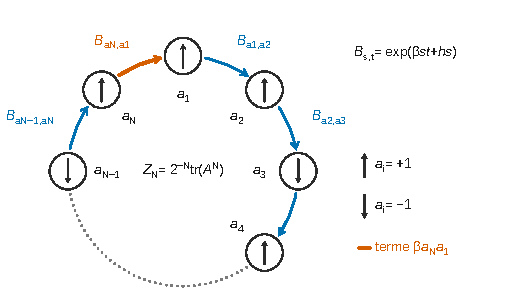
\includegraphics{figures/q12-anneau-transfert.pdf}
\caption*{Figure 2 --- Anneau de spins : chaque lien orienté aᵢ → aᵢ₊₁ porte le
facteur B(aᵢ, aᵢ₊₁), et le terme β a\_N a₁ referme la chaîne, d'où une
trace}
\end{figure}

\hypertarget{question-13}{%
\subsection{Question 13}\label{question-13}}

\begin{indication}{1}

Écrire \(Z_N\) comme une moyenne sur les \(2^N\) configurations, puis reconnaître un coefficient diagonal d'une puissance de matrice.

\end{indication}

\begin{indication}{2}

Attention à l'ordre des lignes et des colonnes : la matrice \((B_{s,t})\) n'est pas exactement \(A\). La trace d'une transposée y remédie.

\end{indication}

\hypertarget{solution-12}{%
\subsubsection{Solution}\label{solution-12}}

\(X^{(N)}\) est uniforme sur \(\{-1,1\}^N\) : par indépendance, chaque configuration \(a\) a la probabilité \(2^{-N}\). Par la formule de transfert et Q12,
\equationajustee{Z_N(\beta,h)=2^{-N}\sum_{a\in\{-1,1\}^N}\Big(\prod_{i=1}^{N-1}B_{a_i,a_{i+1}}\Big)B_{a_N,a_1}.}
(Les facteurs \(B_{\sigma_i,\sigma_{i+1}}\) ne sont pas indépendants : on ne factorise pas l'espérance, on la développe en somme sur les configurations.)

Indexons lignes et colonnes par \((-1,+1)\), dans cet ordre. La matrice \(B=(B_{s,t})\) vaut
\equationajustee{B=\begin{pmatrix}e^{\beta-h}&e^{-\beta-h}\\e^{-\beta+h}&e^{\beta+h}\end{pmatrix}={}^tA .}
Par la formule du produit matriciel,
\equationajustee{(B^N)_{a_1,a_1}=\sum_{a_2,\dots,a_N}B_{a_1,a_2}B_{a_2,a_3}\cdots B_{a_{N-1},a_N}B_{a_N,a_1}.}
En sommant sur \(a_1\), la somme sur les configurations vaut \(\operatorname{tr}(B^N)\). Enfin \(\operatorname{tr}(B^N)=\operatorname{tr}\big({}^t(A^N)\big)=\operatorname{tr}(A^N)\). Donc
\equationajustee{\boxed{Z_N(\beta,h)=2^{-N}\operatorname{tr}(A^N)}}

\begin{jury}

Q13 était difficile : selon le rapport 2026, elle « n'a été que très rarement traitée jusqu'au bout ». Il convenait d'exprimer simultanément la trace et l'espérance en fonction des coefficients \(a_i\).

\end{jury}

\begin{piege}

Factoriser l'espérance d'un produit de facteurs \(B_{\sigma_i,\sigma_{i+1}}\). Le jury le rappelle : ces facteurs ne sont pas mutuellement indépendants (deux facteurs voisins partagent un \(\sigma_i\)). On développe l'espérance en somme sur les \(2^N\) configurations.

\end{piege}

\begin{piege}

Identifier \(A\) à la matrice de transfert sans vérifier les coefficients : ici \(A\) en est la transposée. Il faut le dire, la trace ne voyant pas la différence.

\end{piege}

\hypertarget{question-14}{%
\subsection{Question 14}\label{question-14}}

\begin{indication}{1}

Exprimer \(\operatorname{tr}(A^N)\) avec les valeurs propres, puis comparer leurs modules.

\end{indication}

\begin{indication}{2}

Pour \(\beta\geqslant0\), le signe de \(\det A\) renseigne sur celui de la seconde valeur propre.

\end{indication}

\hypertarget{solution-13}{%
\subsubsection{Solution}\label{solution-13}}

Soit \(\mu\) l'autre valeur propre de \(A\) et \(\lambda=\lambda(\beta,h)\). \(A\) est diagonalisable (deux valeurs propres distinctes en dimension 2), donc \(\operatorname{tr}(A^N)=\lambda^N+\mu^N\).

\emph{Comparaison des modules.} \(\lambda>0\), comme somme de \(e^\beta\operatorname{ch}h>0\) et d'une racine carrée.

Pour \(\beta\geqslant0\), \(\lambda\mu=\det A=2\operatorname{sh}(2\beta)\geqslant0\), donc \(\mu\geqslant0\).

Comme \(\mu<\lambda\) (valeurs propres distinctes, \(\lambda\) la plus grande), on obtient \(0\leqslant\mu/\lambda<1\).

Alors
\equationajustee{F_N(\beta,h)=\ln\lambda-\ln2+\frac1N\ln\Big(1+\big(\tfrac\mu\lambda\big)^N\Big),}
avec
\equationajustee{0\leqslant\frac1N\ln\Big(1+\big(\tfrac\mu\lambda\big)^N\Big)\leqslant\frac{\ln2}N .}
Par encadrement,
\equationajustee{\boxed{\lim_{N\to+\infty}F_N(\beta,h)=\ln\lambda(\beta,h)-\ln2}}

\begin{jury}

Le rapport 2026 : « Beaucoup de candidats ont peu ou mal justifié l'inégalité entre les modules des deux valeurs propres. » Ici, \(\lambda>0\) et \(\lambda\mu=2\operatorname{sh}(2\beta)\geqslant0\) donnent \(0\leqslant\mu<\lambda\) ; sans cela, \(\mu^N\) pourrait ne pas être négligeable.

\end{jury}

\begin{methode}

Contrôle : pour \(\beta=0\), \(\lambda(0,h)=2\operatorname{ch}h\) et l'on retrouve Q9.

\end{methode}

\hypertarget{question-15}{%
\subsection{Question 15}\label{question-15}}

\begin{indication}{1}

Composition de fonctions \(\mathcal C^\infty\) : le seul point à vérifier est que la racine carrée est prise sur une quantité strictement positive.

\end{indication}

\hypertarget{solution-14}{%
\subsubsection{Solution}\label{solution-14}}

D'après Q11, \(\lambda(\beta,h)=e^\beta\operatorname{ch}h+\sqrt{R(\beta,h)}\) avec
\equationajustee{R(\beta,h)=e^{2\beta}\operatorname{sh}^2h+e^{-2\beta}.}
\(R\) est de classe \(\mathcal C^\infty\) sur \(\mathbb R^2\) (sommes, produits et composées de fonctions \(\mathcal C^\infty\)), et \(R\geqslant e^{-2\beta}>0\).

La racine carrée est \(\mathcal C^\infty\) sur \(]0,+\infty[\), donc \(\sqrt R\) l'est aussi.

\textbf{\(\lambda\) est de classe \(\mathcal C^\infty\) sur \(\mathbb R^2\)}, a fortiori sur \([0,+\infty[\times\mathbb R\).

\begin{jury}

Le rapport 2026 attend « quelques justifications (comme par exemple que le terme sous la racine carrée restait strictement positif) ». C'est l'argument décisif : la racine carrée n'est pas dérivable en \(0\).

\end{jury}

\hypertarget{question-16}{%
\subsection{Question 16}\label{question-16}}

\begin{indication}{1}

Montrer d'abord que \(m_N(\beta,h)\) est la dérivée en \(h\) de \(F_N(\beta,h)\).

\end{indication}

\begin{indication}{2}

Appliquer ensuite Q4 à la suite \(h\mapsto F_N(\beta,h)\) : vérifier une par une ses hypothèses à l'aide de Q10, Q14 et Q15.

\end{indication}

\hypertarget{solution-15}{%
\subsubsection{Solution}\label{solution-15}}

Fixons \(\beta\geqslant0\). \(Z_N(\beta,h)=2^{-N}\sum_ae^{H_N(\beta,h,a)}\) est une somme finie de fonctions dérivables en \(h\), avec \(\partial_hH_N(\beta,h,a)=\sum_ia_i\). D'où
\equationajustee{\begin{aligned}
\frac{\partial F_N}{\partial h}(\beta,h)&=\frac1N\,\frac{\partial_hZ_N(\beta,h)}{Z_N(\beta,h)}\\
&=\frac1{Z_N(\beta,h)}E\Big[\Big(\frac1N\sum_{i=1}^N\sigma_i\Big)e^{H_N(\beta,h,X^{(N)})}\Big]\\
&=m_N(\beta,h).
\end{aligned}}
(C'est aussi la première formule de Q7 pour la variable \(Y^{(N)}\) de Q10, coordonnée \(i=2\), divisée par \(N\).)

Posons \(f_N=F_N(\beta,\cdot)\) et vérifions les hypothèses de Q4 :

\begin{itemize}
\tightlist
\item
  chaque \(f_N\) est convexe (restriction à une droite de la fonction convexe \(F_N\), Q10) et dérivable sur \(\mathbb R\) ;
\item
  \((f_N)\) converge simplement vers \(f=\ln\lambda(\beta,\cdot)-\ln2\) (Q14) ;
\item
  \(f\) est dérivable sur \(\mathbb R\) (Q15, et \(\lambda>0\)).
\end{itemize}

La question 4 donne \(f_N'(h)\to f'(h)\), c'est-à-dire
\equationajustee{\boxed{\lim_{N\to+\infty}m_N(\beta,h)=\frac{\partial}{\partial h}\ln\lambda(\beta,h)}}

\begin{jury}

Le rapport 2026 indique que la formule de \(m_N\) découle de Q7 pour une variable bien choisie, et précise : « Le passage à la limite découlait de la question 4 (dont il fallait vérifier les hypothèses). » La liste à puces ci-dessus fait exactement cette vérification.

\end{jury}

\begin{piege}

Dériver « sous la limite » sans justification : l'échange \(\lim_N\) / \(\partial_h\) est exactement ce que fournit Q4, et c'est ce que la question évalue.

\end{piege}

\hypertarget{question-17}{%
\subsection{Question 17}\label{question-17}}

\begin{indication}{1}

Factoriser \(e^\beta\) dans \(\lambda(\beta,h)\) : le \(-\beta\) de \(g_\beta\) sert à cela.

\end{indication}

\begin{indication}{2}

Il reste sous la racine un terme qui tend vers \(0\). Conclure en distinguant le signe de \(h\).

\end{indication}

\hypertarget{solution-16}{%
\subsubsection{Solution}\label{solution-16}}

D'après Q11,
\equationajustee{e^{-\beta}\lambda(\beta,h)=\operatorname{ch}h+\sqrt{\operatorname{sh}^2h+e^{-4\beta}},}
donc
\equationajustee{g_\beta(h)=\ln\Big(\operatorname{ch}h+\sqrt{\operatorname{sh}^2h+e^{-4\beta}}\Big).}
À \(h\) fixé, quand \(\beta\to+\infty\) dans \(\mathbb N\), \(e^{-4\beta}\to0\).

Par continuité de la racine carrée sur \([0,+\infty[\) et du logarithme sur \([1,+\infty[\),
\equationajustee{g_\beta(h)\longrightarrow\ln\big(\operatorname{ch}h+|\operatorname{sh}h|\big).}
Selon le signe de \(h\) : si \(h\geqslant0\), \(\operatorname{ch}h+|\operatorname{sh}h|=\operatorname{ch}h+\operatorname{sh}h=e^h\) ; si \(h<0\), \(\operatorname{ch}h+|\operatorname{sh}h|=\operatorname{ch}h-\operatorname{sh}h=e^{-h}\). Dans les deux cas, la limite vaut \(\ln e^{|h|}=|h|\).

\textbf{\((g_\beta)_{\beta\in\mathbb N}\) converge simplement vers \(h\mapsto|h|\).}

\begin{jury}

Le rapport 2026 attend que l'on justifie les cas possibles selon le signe de \(h\) : \(\operatorname{ch}h+|\operatorname{sh}h|\) vaut \(e^h\) ou \(e^{-h}\) selon ce signe.

\end{jury}

\hypertarget{question-18}{%
\subsection{Question 18}\label{question-18}}

\begin{indication}{1}

On peut calculer explicitement \(g_\beta'\) : le résultat se simplifie beaucoup.

\end{indication}

\begin{indication}{2}

Pour l'uniformité, comparer la régularité des \(g_\beta'\) et celle de leur limite.

\end{indication}

\hypertarget{solution-17}{%
\subsubsection{Solution}\label{solution-17}}

Posons \(c=e^{-4\beta}\) et \(r=\sqrt{\operatorname{sh}^2h+c}>0\), de dérivée \(r'=\frac{\operatorname{sh}h\operatorname{ch}h}{r}\). Alors
\equationajustee{\begin{aligned}
g_\beta'(h)&=\frac{\operatorname{sh}h+\frac{\operatorname{sh}h\operatorname{ch}h}{r}}{\operatorname{ch}h+r}\\
&=\frac{\operatorname{sh}h\,(r+\operatorname{ch}h)}{r\,(\operatorname{ch}h+r)}\\
&=\frac{\operatorname{sh}h}{\sqrt{\operatorname{sh}^2h+e^{-4\beta}}}.
\end{aligned}}
Pour \(h>0\), \(g_\beta'(h)\to\frac{\operatorname{sh}h}{|\operatorname{sh}h|}=1\). Pour \(h<0\), la limite vaut \(-1\). Enfin \(g_\beta'(0)=0\) pour tout \(\beta\). La limite simple est
\equationajustee{\boxed{\ell(h)=\begin{cases}-1&h<0\\0&h=0\\1&h>0\end{cases}}}
Pour \(h\neq0\), on retrouve ce que donne Q4 appliquée aux \(g_\beta\) : elles sont convexes comme limites simples des \(F_N(\beta,\cdot)+\ln2-\beta\) (Q2, Q10, Q14), et \(|\cdot|\) est dérivable en \(h\neq0\) (Q17).

\textbf{La convergence n'est pas uniforme.} Chaque \(g_\beta'\) est continue sur \(\mathbb R\), et une limite uniforme de fonctions continues est continue, ce que \(\ell\) n'est pas en \(0\).

Explicitement, \(g_\beta'(e^{-2\beta})\to\frac1{\sqrt2}\) alors que \(\ell(e^{-2\beta})=1\), donc \(\sup_h|g_\beta'(h)-\ell(h)|\) ne tend pas vers \(0\).

\begin{figure}[H]
\centering
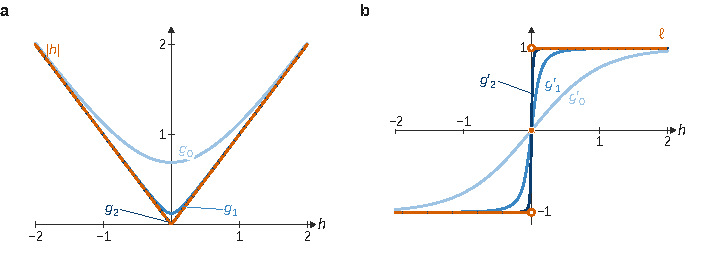
\includegraphics{figures/q18-convergence-derivees.pdf}
\caption*{Figure 3 --- (a) g\_β → \textbar h\textbar{} simplement ; (b) les g\_β′,
continues et nulles en 0, tendent vers ℓ, discontinue en 0 (tracé pour β
= 0, 1, 2)}
\end{figure}

\begin{methode}

Autre voie, celle que décrit le rapport 2026 (qui cite Q2, Q4, Q14 et Q17).

Pour \(h\neq0\) : les \(g_\beta\) sont convexes comme limites simples de fonctions convexes, et \(|\cdot|\) est dérivable en \(h\), donc Q4 s'applique.

En \(h=0\), la parité de \(g_\beta\) donne \(g_\beta'(0)=0\).

\end{methode}

\begin{piege}

Conclure à l'uniformité parce que les \(g_\beta\) convergent vers une fonction « simple ». Autre oubli fréquent : écrire que la limite est la fonction signe sans préciser sa valeur \(\ell(0)=0\).

\end{piege}

\begin{center}\rule{0.5\linewidth}{0.5pt}\end{center}

\hypertarget{partie-iii-champ-moyen-et-transition-de-phase}{%
\section{Partie III --- Champ moyen et transition de phase}\label{partie-iii-champ-moyen-et-transition-de-phase}}

On estime la loi de \(S_N\) à l'échelle exponentielle par Stirling, on étudie les maxima de \(\psi_{\beta,h}=\beta x^2+hx-I(x)\), et l'on en déduit la dérivabilité de l'énergie libre \(g\) et l'aimantation.

\hypertarget{question-19}{%
\subsection{Question 19}\label{question-19}}

\begin{indication}{1}

Un seul type de terme pose problème au bord : de la forme \(u\ln u\) avec \(u\to0^+\).

\end{indication}

\hypertarget{solution-18}{%
\subsubsection{Solution}\label{solution-18}}

Posons \(p=\frac{1+x}2\) et \(q=\frac{1-x}2\), de sorte que \(I(x)=p\ln p+q\ln q\).

Quand \(x\to1^-\), \(p\to1\) donc \(p\ln p\to0\), et \(q\to0^+\) donc \(q\ln q\to0\) (croissances comparées).

\(I\) étant paire, il en va de même en \(-1^+\).

\textbf{\(I\) se prolonge par continuité en posant \(I(\pm1)=0\)}, et devient continue sur \([-1,1]\).

\hypertarget{question-20}{%
\subsection{Question 20}\label{question-20}}

\begin{indication}{1}

L'événement \(\{S_N=x\}\) fixe le nombre de spins égaux à \(+1\) : quelle est la loi de ce nombre ?

\end{indication}

\begin{indication}{2}

Ne pas oublier les valeurs de \(x\) que \(S_N\) ne peut pas prendre.

\end{indication}

\hypertarget{solution-19}{%
\subsubsection{Solution}\label{solution-19}}

Soit \(K\) le nombre d'indices \(i\leqslant N\) tels que \(\sigma_i=1\).

On a \(K=\sum_i\frac{1+\sigma_i}2\), somme de \(N\) variables de Bernoulli de paramètre \(\frac12\) mutuellement indépendantes, donc \(K\sim\mathcal B(N,\frac12)\).

Comme \(\sum_i\sigma_i=K-(N-K)\),
\equationajustee{S_N=\frac{2K-N}N=-1+\frac{2K}N .}
\(S_N\) prend donc ses valeurs dans \(\mathscr M_N\), et \(S_N=x\) équivaut à \(K=\frac{N(1+x)}2\). D'où
\equationajustee{\boxed{P[S_N=x]=\begin{cases}\dbinom{N}{\frac{N(1+x)}2}2^{-N}&\text{si }x\in\mathscr M_N,\\[2mm]0&\text{sinon.}\end{cases}}}

\begin{jury}

Le rapport 2026 : « Il convenait également de préciser pour quelles valeurs de \(x\) la probabilité était nécessairement nulle. » La disjonction \(x\in\mathscr M_N\) ou non fait partie de la réponse.

\end{jury}

\hypertarget{question-21}{%
\subsection{Question 21}\label{question-21}}

\begin{indication}{1}

Appliquer la formule de Stirling aux trois factorielles du coefficient binomial ; seuls les termes de la forme \(n\ln n\) survivent après division par \(N\).

\end{indication}

\begin{indication}{2}

Faire un test en \(x=0\) avant de conclure : \(P[S_N=0]\) décroît-elle exponentiellement ?

\end{indication}

\hypertarget{solution-20}{%
\subsubsection{Solution}\label{solution-20}}

Posons \(m_N=\frac{N(1+u_N)}2\) : comme \(u_N\in\mathscr M_N\), c'est un entier de \(\{0,\dots,N\}\).

Posons aussi \(p_N=\frac{m_N}N=\frac{1+u_N}2\) et \(q_N=1-p_N\).

Alors \(p_N\to p=\frac{1+x}2\in\,]0,1[\) et \(q_N\to q=1-p\).

\emph{Les arguments des factorielles tendent vers l'infini.} \(m_N=Np_N\) et \(N-m_N=Nq_N\) avec \(p,q>0\), donc \(m_N\to+\infty\) et \(N-m_N\to+\infty\).

\emph{Stirling sans sommer d'équivalents.} De \(n!\sim\sqrt{2\pi n}\,(n/e)^n\) on tire, en passant au logarithme (si \(a_n\sim b_n\), alors \(\ln a_n-\ln b_n=\ln\frac{a_n}{b_n}\to0\)) :
\equationajustee{\ln n!=n\ln n-n+\tfrac12\ln(2\pi n)+o(1).}
On l'applique à \(N\), \(m_N\) et \(N-m_N\), qui tendent tous vers l'infini, et on \textbf{soustrait des égalités} (et non des équivalents). Les termes \(-n\) se compensent et les termes \(\frac12\ln(2\pi\,\cdot)\) sont des \(O(\ln N)\) :
\equationajustee{\ln\binom N{m_N}=N\ln N-m_N\ln m_N-(N-m_N)\ln(N-m_N)+O(\ln N).}
Avec \(\ln m_N=\ln N+\ln p_N\) et \(\ln(N-m_N)=\ln N+\ln q_N\), les termes en \(\ln N\) se compensent :
\equationajustee{\begin{aligned}
\frac1N\ln\binom N{m_N}&=-p_N\ln p_N-q_N\ln q_N+O\Big(\frac{\ln N}N\Big)\\
&\longrightarrow-p\ln p-q\ln q=-I(x),
\end{aligned}}
par continuité de \(u\mapsto u\ln u\) sur \(]0,1[\). Par Q20,
\equationajustee{-\frac1N\ln P[S_N=u_N]=-\frac1N\ln\binom N{m_N}+\ln2,}
donc
\equationajustee{\boxed{\lim_{N\to+\infty}-\frac1N\ln P[S_N=u_N]=I(x)+\ln2}}
\textbf{L'énoncé, qui annonce \(I(x)\), comporte une erreur de constante.}

Contrôle en \(x=0\) (avec \(u_N\in\{0,\frac1N\}\)) : \(P[S_N=u_N]\) est de l'ordre de \(\sqrt{2/(\pi N)}\) et ne décroît pas exponentiellement.

La limite vaut donc \(0=I(0)+\ln2\), alors que \(I(0)=-\ln2\). Le résultat annoncé serait exact avec
\equationajustee{J(x)=I(x)+\ln2=\frac{1+x}2\ln(1+x)+\frac{1-x}2\ln(1-x).}

\begin{jury}

Le rapport 2026 confirme l'erratum : « L'énoncé de cette question était erroné, il manquait un terme en \(-\ln(2)\). Cela n'a cependant pas eu d'impact sur les copies ou les corrections puisque ce terme constant ne jouait aucun rôle par la suite. »

\end{jury}

\begin{piege}

Sommer des équivalents. Le jury met en garde : on ne peut pas ajouter les équivalents de Stirling. On passe au logarithme, on écrit des \textbf{égalités} avec des \(o(1)\), et l'on vérifie que les arguments des factorielles tendent vers l'infini.

\end{piege}

\begin{piege}

« Démontrer » le résultat de l'énoncé en perdant le terme \(-N\ln2\) venant de \(2^{-N}\). Quand un calcul honnête contredit l'énoncé, il faut vérifier sur un cas simple, écrire ce que l'on obtient, le signaler en une phrase, puis continuer.

\end{piege}

\hypertarget{question-22}{%
\subsection{Question 22}\label{question-22}}

\begin{indication}{1}

Écrire \(Y_N\) comme une somme finie sur les valeurs de \(S_N\), et minorer cette somme de termes positifs par l'un d'eux.

\end{indication}

\hypertarget{solution-21}{%
\subsubsection{Solution}\label{solution-21}}

Soit \(x\in\mathscr M_N\). \(S_N\) prend ses valeurs dans l'ensemble fini \(\mathscr M_N\), donc, par la formule de transfert,
\equationajustee{Y_N(\beta,h)=\sum_{y\in\mathscr M_N}P[S_N=y]\,e^{N(\beta y^2+hy)} .}
C'est une somme finie de termes positifs, donc elle majore chacun d'eux :
\equationajustee{Y_N(\beta,h)\geqslant P[S_N=x]\,e^{N(\beta x^2+hx)}.}
Comme \(P[S_N=x]>0\) (Q20), on prend le logarithme (croissant) et on divise par \(N\) :
\equationajustee{\boxed{G_N(\beta,h)\geqslant\beta x^2+hx+\frac1N\ln P[S_N=x]}}
Compte tenu de Q21, la convergence admise est exacte sous la forme \(G_N(\beta,h)\to g(\beta,h)-\ln2\), avec \(g\) défini comme dans l'énoncé ; seule cette forme sert en Q30.

\begin{jury}

Question « assez peu difficile mais très peu traitée » selon le rapport 2026 : le point clé était que l'espérance définissant \(Y_N\) est une somme finie de termes positifs. C'est typiquement une question qui départage les copies qui abordent la partie III.

\end{jury}

\begin{methode}

C'est la moitié « facile » de la formule admise.

Pour \(x\in\,]-1,1[\) et une suite \(u_N\in\mathscr M_N\) tendant vers \(x\), Q21 et la continuité de \(y\mapsto\beta y^2+hy\) minorent asymptotiquement \(G_N\) par \(\beta x^2+hx-I(x)-\ln2\).

La majoration (non demandée) vient de ce que la somme compte au plus \(N+1\) termes.

\end{methode}

\hypertarget{question-23}{%
\subsection{Question 23}\label{question-23}}

\begin{indication}{1}

Calculer \(I'\) puis \(I''\) : on obtient une expression très simple.

\end{indication}

\begin{indication}{2}

L'inéquation compare \(2\beta\) à \(\frac1{1-x^2}\), qui vaut au moins \(1\) sur \(]-1,1[\).

\end{indication}

\hypertarget{solution-22}{%
\subsubsection{Solution}\label{solution-22}}

Sur \(]-1,1[\), on dérive les deux termes de \(I\) :
\equationajustee{\begin{aligned}
I'(x)&=\tfrac12\ln\tfrac{1+x}2+\tfrac12-\tfrac12\ln\tfrac{1-x}2-\tfrac12\\
&=\tfrac12\ln\frac{1+x}{1-x},
\end{aligned}}
puis
\equationajustee{\begin{aligned}
I''(x)&=\frac12\Big(\frac1{1+x}+\frac1{1-x}\Big)\\
&=\frac1{1-x^2}.
\end{aligned}}
Donc, indépendamment de \(h\),
\equationajustee{\psi_{\beta,h}''(x)=2\beta-\frac1{1-x^2}.}

\begin{itemize}
\tightlist
\item
  Si \(\beta\in[0,\frac12]\) : \(\frac1{1-x^2}\geqslant1\geqslant2\beta\), donc \textbf{\(\psi''_{\beta,h}(x)\leqslant0\) pour tout \(x\in\,]-1,1[\)} (avec égalité seulement pour \(\beta=\frac12\) et \(x=0\)).
\item
  Si \(\beta>\frac12\) : \(\psi''_{\beta,h}(x)\leqslant0\) équivaut à \(1-x^2\leqslant\frac1{2\beta}\), c'est-à-dire, avec \(x\in\,]-1,1[\), \equationajustee{\boxed{|x|\geqslant\sqrt{1-\frac1{2\beta}}}}
\end{itemize}

\begin{piege}

Le rapport 2026 : « De nombreuses erreurs de calcul sur les dérivées secondes (des problèmes de signes notamment) ont impacté la réussite à cette question et aux deux suivantes. » Contrôle rapide : \(I\) est convexe (c'est une entropie changée de signe), donc \(I''>0\), et \(I''(0)=1\).

\end{piege}

\begin{methode}

Le seuil \(\beta=\frac12\) apparaît ici : pour \(\beta>\frac12\), \(\psi\) est convexe près de \(0\), ce qui annonce que \(0\) cessera d'être le maximum (Q25).

\end{methode}

\hypertarget{question-24}{%
\subsection{Question 24}\label{question-24}}

\begin{indication}{1}

Existence : continuité sur un segment (Q19). Localisation : comparer \(\psi(x)\) et \(\psi(-x)\), puis examiner le signe de \(\psi'\) en \(0\) et au voisinage de \(1\).

\end{indication}

\begin{indication}{2}

Unicité : un point de maximum intérieur annule \(\psi'\). Étudier la concavité de \(\psi'\) sur \([0,1[\) à l'aide de \(\psi'''\).

\end{indication}

\begin{indication}{3}

Une fonction strictement concave, strictement positive en \(0\), ne peut pas s'annuler deux fois sur \(]0,1[\) : écrire le premier zéro comme barycentre de \(0\) et du second.

\end{indication}

\hypertarget{solution-23}{%
\subsubsection{Solution}\label{solution-23}}

Soient \(\beta\geqslant0\) et \(h>0\). \(\psi=\psi_{\beta,h}\) est continue sur le segment \([-1,1]\) (Q19), donc atteint son maximum.

\emph{Localisation.} \(\beta x^2\) et \(I\) sont paires, donc pour \(x\in\,]0,1]\),
\equationajustee{\psi(x)-\psi(-x)=2hx>0 :}
aucun point de \([-1,0[\) n'est point de maximum. Sur \(]-1,1[\),
\equationajustee{\psi'(x)=2\beta x+h-\frac12\ln\frac{1+x}{1-x}.}
- D'une part \(\psi'(0)=h>0\), donc \(\psi\) croît strictement au voisinage de \(0\) : \(0\) n'est pas un maximum.
- D'autre part \(\psi'(x)\to-\infty\) quand \(x\to1^-\). Il existe donc \(a<1\) tel que \(\psi'<0\) sur \([a,1[\).
- Alors \(\psi\), continue en \(1\), est strictement décroissante sur \([a,1]\) : \(1\) n'est pas un maximum.

Tout point de maximum est donc dans l'ouvert \(]0,1[\), où \(\psi\) est dérivable : il annule \(\psi'\).

\emph{Unicité.} Sur \(]0,1[\),
\equationajustee{\psi'''(x)=-I'''(x)=-\frac{2x}{(1-x^2)^2}<0 .}
\(\psi''\) est donc strictement décroissante sur \([0,1[\), et \(\psi'\) y est \textbf{strictement concave} (argument de Q6, avec des inégalités strictes).

Supposons que \(\psi'\) s'annule en \(0<z_1<z_2<1\). Écrivons \(z_1=t\cdot0+(1-t)z_2\) avec \(t\in\,]0,1[\). La stricte concavité donne
\equationajustee{\begin{aligned}
0=\psi'(z_1)&>t\,\psi'(0)+(1-t)\,\psi'(z_2)\\
&=th>0,
\end{aligned}}
ce qui est absurde. \(\psi'\) a donc au plus un zéro dans \(]0,1[\), et au moins un (le point de maximum).

\textbf{\(\psi_{\beta,h}\) atteint son maximum en un unique point \(x_*(\beta,h)\in\,]0,1[\)}, caractérisé par \(\psi'_{\beta,h}(x_*)=0\).

De plus \(\psi'>0\) sur \([0,x_*[\) et \(\psi'<0\) sur \(]x_*,1[\).

\emph{Cas \(h<0\).} On a \(\psi_{\beta,h}(x)=\psi_{\beta,-h}(-x)\). Donc \(\psi_{\beta,h}\) atteint son maximum en un unique point, à savoir \(-x_*(\beta,-h)\in\,]-1,0[\).

\begin{jury}

Le rapport 2026 attendait une étude de fonction ou des arguments de convexité, et précise : « L'argumentation nécessitait d'étudier les cas pour \(\beta\) considérés dans la question précédente. » La preuve ci-dessus évite cette disjonction grâce au signe de \(\psi'''\), valable pour tout \(\beta\geqslant0\) ; la voie par cas est donnée dans l'encadré suivant.

\end{jury}

\begin{methode}

Voie par cas. Si \(\beta\leqslant\frac12\), \(\psi''<0\) sur \(]0,1[\) (Q23) : \(\psi'\) décroît strictement de \(h>0\) vers \(-\infty\) et s'annule une seule fois.

Si \(\beta>\frac12\), \(\psi''\) décroît de \(2\beta-1>0\) vers \(-\infty\) : \(\psi'\) croît, puis décroît strictement vers \(-\infty\).

Elle reste \(>0\) tant qu'elle croît (elle part de \(h>0\)), puis s'annule une seule fois.

\end{methode}

\begin{piege}

Montrer seulement l'existence d'un point critique. La question demande l'\textbf{unicité} du point de maximum ; l'existence d'un zéro de \(\psi'\) ne suffit pas.

\end{piege}

\hypertarget{question-25}{%
\subsection{Question 25}\label{question-25}}

\begin{indication}{1}

\(\psi_{\beta,0}\) est paire et \(0\) est un point critique. Pour \(\beta\leqslant\frac12\), utiliser Q23.

\end{indication}

\begin{indication}{2}

Pour \(\beta>\frac12\) : que dit le signe de \(\psi''_{\beta,0}(0)\) ? Reprendre ensuite l'argument de concavité stricte de \(\psi'\) sur \([0,1[\) (Q24), en tenant compte du zéro déjà connu en \(0\).

\end{indication}

\hypertarget{solution-24}{%
\subsubsection{Solution}\label{solution-24}}

Ici \(h=0\) : \(\psi_{\beta,0}(x)=\beta x^2-I(x)\) est paire et \(\psi'_{\beta,0}(0)=0\).

\emph{Cas \(\beta\in[0,\frac12]\).} Par Q23, \(\psi''_{\beta,0}<0\) sur \(]-1,1[\), sauf éventuellement en \(0\).

\(\psi'_{\beta,0}\) est donc strictement décroissante. Nulle en \(0\), elle est \(>0\) sur \(]-1,0[\) et \(<0\) sur \(]0,1[\).

Par continuité de \(\psi_{\beta,0}\) en \(\pm1\), \(\psi_{\beta,0}\) est strictement croissante sur \([-1,0]\) et strictement décroissante sur \([0,1]\).

\textbf{Le maximum est atteint en \(0\) et seulement en \(0\).}

\emph{Cas \(\beta>\frac12\).} Sur \([0,1[\), \(\psi'_{\beta,0}\) est strictement concave (même calcul qu'en Q24). On dispose de :

\begin{itemize}
\tightlist
\item
  \(\psi'_{\beta,0}(0)=0\) et \(\psi''_{\beta,0}(0)=2\beta-1>0\), donc il existe \(\varepsilon\in\,]0,1[\) avec \(\psi'_{\beta,0}(\varepsilon)>0\) ;
\item
  \(\psi'_{\beta,0}(x)\to-\infty\) quand \(x\to1^-\).
\end{itemize}

Par le théorème des valeurs intermédiaires, \(\psi'_{\beta,0}\) s'annule en un point \(c\in\,]\varepsilon,1[\).

Ce zéro est unique dans \(]0,1[\).

En effet, une fonction strictement concave s'annule au plus deux fois : si \(a<b<c'\) étaient trois zéros, \(b\) serait combinaison convexe stricte de \(a\) et \(c'\), et la stricte concavité donnerait \(0>0\). Or \(0\) est déjà un zéro.

Entre ses zéros, \(\psi'_{\beta,0}\) garde un signe constant (valeurs intermédiaires). Elle est \(>0\) en \(\varepsilon<c\) et tend vers \(-\infty\) en \(1^-\).

Donc \(\psi'_{\beta,0}>0\) sur \(]0,c[\) et \(\psi'_{\beta,0}<0\) sur \(]c,1[\).

Ainsi \(\psi_{\beta,0}\) est strictement croissante sur \([0,c]\) et strictement décroissante sur \([c,1]\) : sur \([0,1]\), le maximum est atteint en \(c\) seul.

Par parité, sur \([-1,1]\), \textbf{le maximum est atteint exactement en \(x_*(\beta,0):=c\in\,]0,1[\) et en \(-x_*(\beta,0)\).}

\begin{figure}[H]
\centering
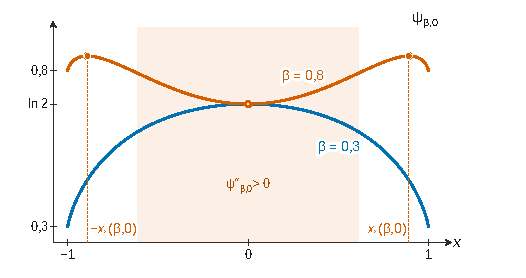
\includegraphics{figures/q25-profil-psi.pdf}
\caption*{Figure 4 --- Profil ψ\_β,0 : maximum unique en 0 pour β = 0,3 ; pour β =
0,8, 0 devient un minimum local (zone teintée : ψ″ \textgreater{} 0) et
les maxima sont en ±x*(β, 0)}
\end{figure}

\begin{methode}

Interprétation : pour \(\beta>\frac12\) (basse température), le profil \(\psi_{\beta,0}\) a deux bosses symétriques, et le système choisit une aimantation \(\pm x_*(\beta,0)\neq0\) en l'absence de champ.

\end{methode}

\hypertarget{question-26}{%
\subsection{Question 26}\label{question-26}}

\begin{indication}{1}

Écrire l'inégalité qui caractérise \(x_*(\beta,v_n)\) comme point de maximum, pour tout \(y\in[-1,1]\), puis passer à la limite.

\end{indication}

\begin{indication}{2}

Conclure par l'unicité de Q24.

\end{indication}

\hypertarget{solution-25}{%
\subsubsection{Solution}\label{solution-25}}

Comme \(v_n\to h>0\), il existe \(n_1\) tel que \(v_n>0\) pour \(n\geqslant n_1\).

Posons alors \(x_n=x_*(\beta,v_n)\in\,]0,1[\) et \(\ell=\lim x_n\), qui appartient au fermé \([0,1]\).

\emph{Caractère maximal.} Pour \(n\geqslant n_1\) et tout \(y\in[-1,1]\),
\equationajustee{\beta x_n^2+v_nx_n-I(x_n)\geqslant\beta y^2+v_ny-I(y).}

\emph{Passage à la limite.} \(I\) est continue sur \([-1,1]\) (Q19), y compris aux bords, où \(\ell\) peut se trouver a priori. Avec \(x_n\to\ell\) et \(v_n\to h\), on obtient, pour tout \(y\in[-1,1]\),
\equationajustee{\psi_{\beta,h}(\ell)\geqslant\psi_{\beta,h}(y).}

\emph{Unicité.} \(\ell\) est un point de maximum de \(\psi_{\beta,h}\) ; par l'unicité de Q24,
\equationajustee{\boxed{\lim_{n\to\infty}x_*(\beta,v_n)=x_*(\beta,h)}}

\begin{jury}

Selon le rapport 2026, cette question « très peu traitée et assez subtile » demandait d'utiliser « avec soin le caractère maximal de \(x_*(\beta, h)\), l'unicité du maximum et un argument de passage à la limite soigneux ». Ce sont les trois étapes en italique de la solution.

\end{jury}

\begin{piege}

Oublier de dire que la limite \(\ell\) reste dans \([-1,1]\) (fermé) et que \(I\) est continue jusqu'au bord : c'est Q19 qui sert ici.

\end{piege}

\hypertarget{question-27}{%
\subsection{Question 27}\label{question-27}}

\begin{indication}{1}

\(g(\beta,h')\) est un supremum : il majore \(\psi_{\beta,h'}\) en tout point, en particulier en un point bien choisi.

\end{indication}

\begin{indication}{2}

Évaluer en \(x_*(\beta,h)\) et faire apparaître \(\psi_{\beta,h}(x_*(\beta,h))\) ; puis échanger les rôles de \(h\) et \(h'\).

\end{indication}

\hypertarget{solution-26}{%
\subsubsection{Solution}\label{solution-26}}

Pour \(h\geqslant0\), \(x_*(\beta,h)\) est un point de maximum de \(\psi_{\beta,h}\) sur \([-1,1]\).

C'est Q24 si \(h>0\), et Q25 si \(h=0\), que \(\beta\) soit au-dessous ou au-dessus de \(\frac12\).

Le supremum \(g(\beta,h)\) est donc atteint :
\equationajustee{g(\beta,h)=\psi_{\beta,h}\big(x_*(\beta,h)\big).}
Posons \(x_*=x_*(\beta,h)\) et comparons \(\psi_{\beta,h'}\) et \(\psi_{\beta,h}\) : \(\psi_{\beta,h'}(x)=\psi_{\beta,h}(x)+(h'-h)x\). Comme \(g(\beta,h')\) majore \(\psi_{\beta,h'}\),
\equationajustee{\begin{aligned}
g(\beta,h')&\geqslant\psi_{\beta,h'}(x_*)\\
&=\psi_{\beta,h}(x_*)+(h'-h)x_*\\
&=g(\beta,h)+(h'-h)x_*.
\end{aligned}}
En échangeant les rôles de \(h\) et \(h'\) :
\equationajustee{g(\beta,h)\geqslant g(\beta,h')+(h-h')\,x_*(\beta,h').}
D'où
\equationajustee{\boxed{(h'-h)\,x_*(\beta,h)\leqslant g(\beta,h')-g(\beta,h)\leqslant(h'-h)\,x_*(\beta,h')}}

\begin{jury}

Question « très peu traitée quoique pas extrêmement difficile », selon le rapport 2026, qui attend là encore le caractère maximal de \(x_*(\beta,h)\) et une comparaison explicite des formules de \(\psi_{\beta,h'}\) et \(\psi_{\beta,h}\). L'identité \(\psi_{\beta,h'}(x)=\psi_{\beta,h}(x)+(h'-h)x\) fait tout le travail.

\end{jury}

\begin{methode}

Un supremum de fonctions affines de \(h\) est convexe, et chaque fonction affine qui le réalise en un point est une droite d'appui : on obtient des inégalités de pente sans rien dériver.

\end{methode}

\hypertarget{question-28}{%
\subsection{Question 28}\label{question-28}}

\begin{indication}{1}

Diviser l'encadrement de Q27 par \(h'-h\) en distinguant le signe de \(h'-h\).

\end{indication}

\begin{indication}{2}

Utiliser la continuité admise de \(h\mapsto x_*(\beta,h)\) et le théorème d'encadrement.

\end{indication}

\hypertarget{solution-27}{%
\subsubsection{Solution}\label{solution-27}}

Soit \(h>0\) et \(h'\geqslant0\) avec \(h'\neq h\). On divise l'encadrement de Q27 par \(h'-h\), en renversant les inégalités si \(h'<h\) : le taux
\equationajustee{\tau(h')=\frac{g(\beta,h')-g(\beta,h)}{h'-h}}
est compris entre \(x_*(\beta,h)\) et \(x_*(\beta,h')\).

Par la continuité admise de \(h'\mapsto x_*(\beta,h')\) sur \([0,+\infty[\), \(x_*(\beta,h')\to x_*(\beta,h)\) quand \(h'\to h\).

Par encadrement, \(\tau(h')\to x_*(\beta,h)\) :
\equationajustee{\boxed{h'\mapsto g(\beta,h')\text{ est \text{dérivable} en }h\text{ et }\frac{\partial g}{\partial h}(\beta,h)=x_*(\beta,h)}}

\begin{jury}

Le rapport 2026 note que cette question a été bien plus traitée que la précédente : elle n'utilise essentiellement que la continuité de \(h\mapsto x_*(\beta,h)\). On peut admettre Q27 pour la traiter.

\end{jury}

\hypertarget{question-29}{%
\subsection{Question 29}\label{question-29}}

\begin{indication}{1}

Montrer que \(g(\beta,\cdot)\) est paire ; seul le point \(h=0\) reste à étudier.

\end{indication}

\begin{indication}{2}

Calculer la dérivée à droite en \(0\) par Q27 avec \(h=0\) ; en déduire la dérivée à gauche par parité, puis utiliser Q25.

\end{indication}

\hypertarget{solution-28}{%
\subsubsection{Solution}\label{solution-28}}

\emph{Parité.} \(\psi_{\beta,-h}(x)=\psi_{\beta,h}(-x)\) et \([-1,1]\) est symétrique, donc \(g(\beta,-h)=g(\beta,h)\).

\emph{Hors de \(0\).} \(g(\beta,\cdot)\) est dérivable sur \(]0,+\infty[\) (Q28), donc sur \(]-\infty,0[\) par parité (composée avec \(h\mapsto-h\)).

\emph{En \(0\).} Q27 avec \(h=0\) et \(h'>0\) donne
\equationajustee{x_*(\beta,0)\leqslant\frac{g(\beta,h')-g(\beta,0)}{h'}\leqslant x_*(\beta,h').}
Par la continuité admise en \(0\), la dérivée à droite en \(0\) existe et vaut \(x_*(\beta,0)\). Par parité, la dérivée à gauche vaut \(-x_*(\beta,0)\).

Donc \(g(\beta,\cdot)\) est dérivable en \(0\) si et seulement si \(x_*(\beta,0)=0\), c'est-à-dire, par Q25, si et seulement si \(\beta\leqslant\frac12\) :
\equationajustee{\boxed{h\mapsto g(\beta,h)\text{ est \text{dérivable} sur }\mathbb R\iff\beta\in\big[0,\tfrac12\big]}}

\begin{figure}[H]
\centering
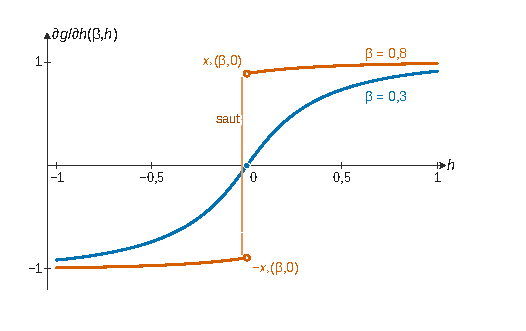
\includegraphics{figures/q29-aimantation-saut.pdf}
\caption*{Figure 5 --- Dérivée ∂g/∂h (β, h) en fonction de h : continue pour β =
0,3, saut de −x\emph{(β, 0) à x}(β, 0) en h = 0 pour β = 0,8}
\end{figure}

\begin{jury}

Question très peu traitée ; le rapport 2026 situe sa difficulté en \(h=0\). Hors de \(0\), tout découle de Q28 et de la parité.

\end{jury}

\begin{methode}

C'est la transition de phase : pour \(\beta>\frac12\), l'aimantation \(\partial_hg\) saute de \(-x_*(\beta,0)\) à \(x_*(\beta,0)\) en \(h=0\). On retrouve le « coin » de \(|h|\) vu en Q17--Q18.

\end{methode}

\hypertarget{question-30}{%
\subsection{Question 30}\label{question-30}}

\begin{indication}{1}

Simplifier la double somme \(\sum_{i,j}\sigma_i\sigma_j\) et reconnaître dans la quantité une dérivée de \(G_N\).

\end{indication}

\begin{indication}{2}

Vérifier les hypothèses de Q4 pour la suite \(G_N(\beta,\cdot)\) : convexité (partie I), dérivabilité, limite simple (admise), dérivabilité de la limite en \(h>0\) (Q28).

\end{indication}

\hypertarget{solution-29}{%
\subsubsection{Solution}\label{solution-29}}

On a \(\frac\beta N\sum_{i,j}\sigma_i\sigma_j=\frac\beta N\big(\sum_i\sigma_i\big)^2=\beta NS_N^2\) et \(h\sum_i\sigma_i=hNS_N\). La quantité étudiée vaut donc
\equationajustee{Q_N=\frac{E\big[S_N\,e^{\beta NS_N^2+hNS_N}\big]}{Y_N(\beta,h)} .}
\(Y_N\) est une somme finie de fonctions dérivables en \(h\) (Q22), et
\equationajustee{\begin{aligned}
Q_N&=\frac1N\,\frac{\partial_hY_N(\beta,h)}{Y_N(\beta,h)}\\
&=\frac{\partial G_N}{\partial h}(\beta,h).
\end{aligned}}
Vérifions les hypothèses de Q4 pour \(f_N=G_N(\beta,\cdot)+\ln2\) :

\begin{itemize}
\tightlist
\item
  avec \(W^{(N)}=(NS_N^2,NS_N)\), à valeurs dans un ensemble fini de \(\mathbb R^2\), \(\ln Y_N(\beta,h)=\phi_{W^{(N)}}(\beta,h)\) est convexe (Q8) ; donc \(f_N\) est convexe et dérivable sur \(\mathbb R\) ;
\item
  par la convergence admise, sous sa forme rectifiée (Q21--Q22), \(f_N\to g(\beta,\cdot)\) simplement sur \(\mathbb R\) ;
\item
  \(g(\beta,\cdot)\) est dérivable en \(h>0\), de dérivée \(x_*(\beta,h)\) (Q28).
\end{itemize}

La question 4 donne \(f_N'(h)=Q_N\to x_*(\beta,h)\) :
\equationajustee{\boxed{\lim_{N\to+\infty}\frac1{Y_N(\beta,h)}E\Big[\Big(\frac1N\sum_{i=1}^N\sigma_i\Big)\exp\Big(\frac\beta N\sum_{i,j}\sigma_i\sigma_j+h\sum_i\sigma_i\Big)\Big]=x_*(\beta,h)}}
La constante \(\ln2\) est sans effet : l'énoncé tel qu'admis conduirait à la même dérivée.

\begin{jury}

Le rapport 2026 situe la difficulté principale dans le rappel des notations et des résultats antérieurs. Il faut reconnaître \(\partial_hG_N\), puis citer Q8, la convergence admise, Q28 et Q4.

\end{jury}

\begin{piege}

Croire que l'erreur de constante de Q21 change la réponse : une constante additive ne modifie pas la dérivée, et Q4 s'applique aussi bien à \(G_N\) qu'à \(G_N+\ln2\).

\end{piege}

\hypertarget{question-31}{%
\subsection{Question 31}\label{question-31}}

\begin{indication}{1}

Le maximum est intérieur (Q24) : écrire la condition du premier ordre.

\end{indication}

\begin{indication}{2}

Résoudre \(\operatorname{th}t=x\) en \(t\), pour \(x\in\,]-1,1[\).

\end{indication}

\hypertarget{solution-30}{%
\subsubsection{Solution}\label{solution-30}}

Par Q24, \(x_*=x_*(\beta,h)\in\,]0,1[\) annule \(\psi'_{\beta,h}\) :
\equationajustee{\frac12\ln\frac{1+x_*}{1-x_*}=h+2\beta x_* .}
Or, pour \(t\in\mathbb R\) et \(x\in\,]-1,1[\),
\equationajustee{\begin{aligned}
\operatorname{th}t=x&\iff\frac{e^{2t}-1}{e^{2t}+1}=x\\
&\iff e^{2t}=\frac{1+x}{1-x}\\
&\iff t=\frac12\ln\frac{1+x}{1-x}.
\end{aligned}}
Avec \(t=h+2\beta x_*\) :
\equationajustee{\boxed{x_*(\beta,h)=\operatorname{th}\big(h+2\beta x_*(\beta,h)\big)}}

\begin{figure}[H]
\centering
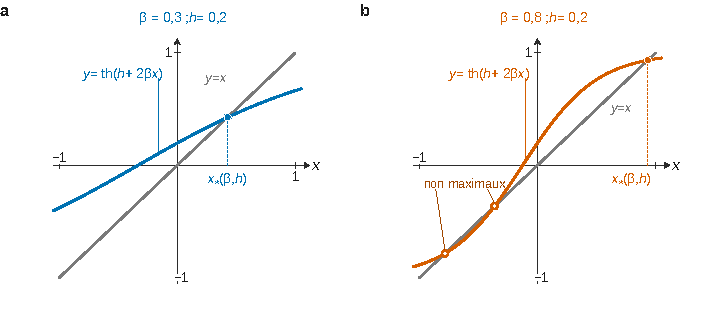
\includegraphics{figures/q31-point-fixe.pdf}
\caption*{Figure 6 --- Pour h = 0,2, x*(β, h) est l'abscisse de l'intersection
positive de y = x et y = th(h + 2βx) ; pour β = 0,8, les deux
intersections négatives ne sont pas des maxima}
\end{figure}

\begin{jury}

Question « peu abordée, mais qui ne nécessitait que très peu de résultats intermédiaires », selon le rapport 2026 : le point de maximum annule la dérivée de \(\psi\), puis un peu de trigonométrie hyperbolique conclut. À ne pas laisser passer, même sans avoir traité Q24 (on l'admet).

\end{jury}

\begin{methode}

C'est l'équation de champ moyen de Curie--Weiss : l'aimantation est celle d'un spin isolé soumis au champ effectif \(h+2\beta x_*\). Graphiquement, \(x_*\) est l'intersection \textbf{positive} des deux courbes de la figure 6 ; l'équation seule ne suffit pas, il faut la localisation de Q24.

\end{methode}

\hypertarget{question-32}{%
\subsection{Question 32}\label{question-32}}

\begin{indication}{1}

À \(\beta=\frac12\), l'équation de Q31 équivaut à \(\Phi(x_*)=h\) pour une fonction \(\Phi\) explicite : étudier \(\Phi\) au voisinage de \(0\).

\end{indication}

\begin{indication}{2}

Il faut d'abord établir que \(x_*(\frac12,h)\to0\) quand \(h\to0^+\), par la monotonie de \(\Phi\) ou par la continuité admise.

\end{indication}

\begin{indication}{3}

Le terme linéaire du développement de \(\frac12\ln\frac{1+x}{1-x}\) se simplifie : c'est le terme d'ordre \(3\) qui donne l'équivalent.

\end{indication}

\hypertarget{solution-31}{%
\subsubsection{Solution}\label{solution-31}}

Notons \(x_h=x_*(\frac12,h)\) pour \(h>0\). Par Q24 et Q31, \(x_h\in\,]0,1[\) et \(\frac12\ln\frac{1+x_h}{1-x_h}=h+x_h\), soit \(\Phi(x_h)=h\) avec
\equationajustee{\Phi(x)=\frac12\ln\frac{1+x}{1-x}-x .}

\emph{\(x_h\) tend vers \(0\).} Sur \(]0,1[\),
\equationajustee{\Phi'(x)=\frac1{1-x^2}-1=\frac{x^2}{1-x^2}>0 .}
\(\Phi\) est donc une bijection continue strictement croissante de \([0,1[\) sur \([0,+\infty[\) (car \(\Phi(0)=0\) et \(\Phi\to+\infty\) en \(1\)), de réciproque continue.

Donc \(x_h=\Phi^{-1}(h)\to\Phi^{-1}(0)=0\) quand \(h\to0^+\).

(On peut aussi invoquer la continuité admise et \(x_*(\frac12,0)=0\), par Q25.)

\emph{Équivalent.} Par différence des développements en série entière de \(\ln(1+x)\) et \(\ln(1-x)\), pour \(|x|<1\),
\equationajustee{\frac12\ln\frac{1+x}{1-x}=\sum_{k\geqslant0}\frac{x^{2k+1}}{2k+1}.}
Donc \(\Phi(x)=\frac{x^3}3+O(x^5)\), d'où \(\Phi(x)\sim\frac{x^3}3\) en \(0\).

Comme \(x_h\to0\), on peut composer : \(h=\Phi(x_h)\sim\frac{x_h^3}3\), soit \(\frac{x_h^3}{3h}\to1\).

Par continuité de \(t\mapsto t^{1/3}\) en \(1\) :
\equationajustee{\boxed{\lim_{\substack{h\to0\\h>0}}\frac{x_*(\frac12,h)}{(3h)^{1/3}}=1}}

\begin{jury}

Le rapport 2026 : la question se déduisait de la précédente par un développement limité, « une fois démontré (ou admis) que \(x_{*}(1/2, h)\) tendait vers 0 en \(h = 0\) ». Cette étape préalable doit apparaître dans la copie.

\end{jury}

\begin{piege}

Composer un équivalent par une fonction sans justification. Ici, on passe de \(\frac{x_h^3}{3h}\to1\) à \(\frac{x_h}{(3h)^{1/3}}\to1\) par continuité de la racine cubique en \(1\), ce qui est licite. Il faut aussi avoir établi \(x_h\to0\) \textbf{avant} d'utiliser le développement en \(0\).

\end{piege}

\begin{methode}

Au point critique \(\beta=\frac12\), le terme linéaire de l'équation se compense exactement et l'aimantation varie comme \(h^{1/3}\) (exposant critique \(\frac13\)). Pour \(\beta<\frac12\), elle varie au contraire comme \(\frac{h}{1-2\beta}\).

\end{methode}

\begin{center}\rule{0.5\linewidth}{0.5pt}\end{center}

\hypertarget{bilan}{%
\section{Bilan}\label{bilan}}

\textbf{Méthodes à retenir.}

\begin{itemize}
\tightlist
\item
  \textbf{Croissance des pentes} d'une fonction convexe (Q1), et sa conséquence majeure : \textbf{la dérivée d'une limite simple de fonctions convexes est la limite des dérivées}, là où la limite est dérivable (Q4). Rédiger en \(\varepsilon\), en choisissant \(h\) avant \(n\).
\item
  \textbf{Restriction à une droite} pour passer de la dimension \(d\) à la dimension 1 (Q5--Q6).
\item
  \textbf{\(\ln E[e^{\lambda\cdot X}]\) est convexe} car sa hessienne est une covariance (Q8) ; toute fonction qui s'écrit ainsi hérite gratuitement de la convexité (Q10, Q30).
\item
  \textbf{Matrice de transfert} : une somme sur des configurations cycliques de produits de coefficients est la trace d'une puissance de matrice (Q13), dominée par la plus grande valeur propre (Q14).
\item
  \textbf{Stirling} pour l'ordre exponentiel d'un coefficient binomial (Q21) : \(\frac1N\ln\binom N{pN}\to-p\ln p-(1-p)\ln(1-p)\). Passer au logarithme et sommer des égalités, jamais des équivalents.
\item
  \textbf{Unicité d'un maximum} par stricte concavité de la dérivée (Q24--Q25) : une fonction strictement concave a au plus deux zéros.
\item
  \textbf{Supremum de fonctions affines} : encadrement des accroissements par les points de maximum, puis dérivabilité par continuité de ces points (Q27--Q29).
\end{itemize}

\textbf{Ce que le jury 2026 a sanctionné.} Des définitions approximatives (matrice symétrique positive en Q5--Q6), des limites dont on n'a pas établi l'existence (Q4), des hypothèses de Q4 non vérifiées (Q16, Q30), l'inégalité entre les modules des valeurs propres (Q14), des erreurs de signe dans les dérivées secondes (Q23). Il rappelle aussi qu'une question précédente utilisée doit être citée explicitement.

\textbf{Questions discriminantes.} Q13 (rarement menée à terme), puis les questions accessibles mais délaissées de la partie III : Q22, Q27 et Q31. Les questions de rigueur Q4, Q26 et Q29 séparent ensuite les meilleures copies.

\textbf{Prérequis à revoir.} Théorème des accroissements finis, théorème de Schwarz, matrices \(2\times2\) (trace, déterminant, diagonalisabilité), loi binomiale, formule de transfert, croissances comparées, convergence simple et uniforme (une limite uniforme de fonctions continues est continue), séries entières usuelles.

\textbf{Questions transposables.} Q1--Q4 (convexité et dérivées) et Q5--Q6 (hessienne) sont des classiques de tout problème d'analyse convexe. Q13--Q14 (trace d'une puissance et valeur propre dominante) se retrouvent dans les chaînes de Markov et le dénombrement de mots. Q21 (Stirling pour un coefficient binomial) est un passage obligé des problèmes de probabilités asymptotiques. Q18 (non-uniformité par discontinuité de la limite) est un réflexe standard.

\textbf{Leçon de l'erratum.} Un test sur un cas simple (\(x=0\) en Q21, \(\beta=0\) en Q14) détecte immédiatement une erreur de constante, dans sa propre copie comme dans un énoncé.

\end{document}
